\documentclass[preprint, 3p,
authoryear]{elsarticle} %review=doublespace preprint=single 5p=2 column
%%% Begin My package additions %%%%%%%%%%%%%%%%%%%

\usepackage[hyphens]{url}

  \journal{An awesome journal} % Sets Journal name

\usepackage{graphicx}
%%%%%%%%%%%%%%%% end my additions to header

\usepackage[T1]{fontenc}
\usepackage{lmodern}
\usepackage{amssymb,amsmath}
% TODO: Currently lineno needs to be loaded after amsmath because of conflict
% https://github.com/latex-lineno/lineno/issues/5
\usepackage{lineno} % add
\usepackage{ifxetex,ifluatex}
\usepackage{fixltx2e} % provides \textsubscript
% use upquote if available, for straight quotes in verbatim environments
\IfFileExists{upquote.sty}{\usepackage{upquote}}{}
\ifnum 0\ifxetex 1\fi\ifluatex 1\fi=0 % if pdftex
  \usepackage[utf8]{inputenc}
\else % if luatex or xelatex
  \usepackage{fontspec}
  \ifxetex
    \usepackage{xltxtra,xunicode}
  \fi
  \defaultfontfeatures{Mapping=tex-text,Scale=MatchLowercase}
  \newcommand{\euro}{€}
\fi
% use microtype if available
\IfFileExists{microtype.sty}{\usepackage{microtype}}{}

\ifxetex
  \usepackage[setpagesize=false, % page size defined by xetex
              unicode=false, % unicode breaks when used with xetex
              xetex]{hyperref}
\else
  \usepackage[unicode=true]{hyperref}
\fi
\hypersetup{breaklinks=true,
            bookmarks=true,
            pdfauthor={},
            pdftitle={A Historical Analysis of the Evolution of Active Travel Behaviour in Canada},
            colorlinks=false,
            urlcolor=blue,
            linkcolor=magenta,
            pdfborder={0 0 0}}

\setcounter{secnumdepth}{5}
% Pandoc toggle for numbering sections (defaults to be off)


% tightlist command for lists without linebreak
\providecommand{\tightlist}{%
  \setlength{\itemsep}{0pt}\setlength{\parskip}{0pt}}


% Pandoc citation processing
\newlength{\cslhangindent}
\setlength{\cslhangindent}{1.5em}
\newlength{\csllabelwidth}
\setlength{\csllabelwidth}{3em}
\newlength{\cslentryspacingunit} % times entry-spacing
\setlength{\cslentryspacingunit}{\parskip}
% for Pandoc 2.8 to 2.10.1
\newenvironment{cslreferences}%
  {}%
  {\par}
% For Pandoc 2.11+
\newenvironment{CSLReferences}[2] % #1 hanging-ident, #2 entry spacing
 {% don't indent paragraphs
  \setlength{\parindent}{0pt}
  % turn on hanging indent if param 1 is 1
  \ifodd #1
  \let\oldpar\par
  \def\par{\hangindent=\cslhangindent\oldpar}
  \fi
  % set entry spacing
  \setlength{\parskip}{#2\cslentryspacingunit}
 }%
 {}
\usepackage{calc}
\newcommand{\CSLBlock}[1]{#1\hfill\break}
\newcommand{\CSLLeftMargin}[1]{\parbox[t]{\csllabelwidth}{#1}}
\newcommand{\CSLRightInline}[1]{\parbox[t]{\linewidth - \csllabelwidth}{#1}\break}
\newcommand{\CSLIndent}[1]{\hspace{\cslhangindent}#1}


\usepackage{booktabs}
\usepackage{longtable}
\usepackage{array}
\usepackage{multirow}
\usepackage{wrapfig}
\usepackage{float}
\usepackage{colortbl}
\usepackage{pdflscape}
\usepackage{tabu}
\usepackage{threeparttable}
\usepackage{threeparttablex}
\usepackage[normalem]{ulem}
\usepackage{makecell}
\usepackage{xcolor}



\begin{document}


\begin{frontmatter}

  \title{A Historical Analysis of the Evolution of Active Travel
Behaviour in Canada}
    \author[Some Institute of Technology]{Alice Anonymous%
  \corref{cor1}%
  \fnref{1}}
   \ead{alice@example.com} 
    \author[Another University]{Bob Security%
  %
  }
   \ead{bob@example.com} 
    \author[Another University]{Cat Memes%
  %
  \fnref{2}}
   \ead{cat@example.com} 
    \author[Some Institute of Technology]{Derek Zoolander%
  %
  \fnref{2}}
   \ead{derek@example.com} 
      \affiliation[Some Institute of Technology]{
    organization={Big Wig University},addressline={1 main
street},city={Gotham},postcode={123456},state={State},country={United
States},}
    \affiliation[Another University]{
    organization={Department},addressline={A street
29},city={Manchester,},postcode={2054 NX},country={The Netherlands},}
    \cortext[cor1]{Corresponding author}
    \fntext[1]{This is the first author footnote.}
    \fntext[2]{Another author footnote.}
  
  \begin{abstract}
  This is the abstract.

  It consists of two paragraphs.
  \end{abstract}
    \begin{keyword}
    keyword1 \sep 
    keyword2
  \end{keyword}
  
 \end{frontmatter}

\hypertarget{introduction}{%
\section{Introduction}\label{introduction}}

The idea that travel behaviour can be influenced by the city form has
attracted growing interest urban and transportation planning. Cities
intend to encourage their residents to adopt more sustainable modes of
transportation, including walking, cycling, and public transit, by
developing an environment with a variety of transportation alternatives
and, at the same time, increasing accessibility - understood as the ease
of reaching destinations and opportunities (Iacono, Krizek, and
El-Geneidy 2008). Because of their significant role in enhancing and
promoting urban sustainability (Hino et al. 2014; Lamiquiz and
Lopez-Dominguez 2015), active transportation modes, such as walking and
cycling, are playing a central role in urban mobility research and
policy-making (S. Handy 1993; Clifton and Handy 2001; Frank and Engelke
2001; Krizek 2005; Sallis et al. 2004; Vandenbulcke, Steenberghen, and
Thomas 2009; Wu et al. 2019). Walking and cycling accessibility are
closely related, contributing together to the concept of ``active
accessibility'' or ``non-motorized accessibility'', and, when considered
in the urban and transportation planning process, reducing dependence on
private vehicles and promoting healthier and more sustainable travel
behaviour among residents.

There are two main components when measuring accessibility: (1) the
location and power of attraction of urban opportunities (trip benefit)
and (2) the barrier in travel from the origin in the network to the
destination (trip cost). A way for measuring the cost of travel when
calculating accessibility is using impedance functions, a methods that
is receiving attention from transportation planning scholars, urban
geography, and sustainable development (Frank et al. 2005; Krizek 2005;
Currie 2010; Iacono, Krizek, and El-Geneidy 2010; Yang and Diez-Roux
2012; Millward, Spinney, and Scott 2013; Nassir et al. 2016; Saghapour,
Moridpour, and Thompson 2017; Wu et al. 2019). The impedance functions
have different forms and all of them serve as a tool to understand the
travel behaviour and as measure of the willingness to travel a certain
distance to achieve a desired destination, where a service or an
opportunity is located (Taylor 1975; Fotheringham 1981; Kwan 1998;
Eldridge and Jones III 1991; Luoma, Mikkonen, and Palomaki 1993; Papa
and Coppola 2012; Yang and Diez-Roux 2012; Millward, Spinney, and Scott
2013; Vale and Pereira 2017). In this concept, areas with higher
accessibility are those characterized by a lower impedance when
traveling to desirable destinations. When talking about active
accessibility, increasing the distance between two points generally
implies in a decreasing in the probability of that trip being done by
walking or biking (Hansen 1959; Pirie 1979; S. L. Handy and Niemeier
1997; K. T. Geurs and Ritsema van Eck 2001; Bhat et al. 2002; Church and
Marston 2003; Kwan et al. 2003; K. T. Geurs and Van Wee 2004; Levinson
and Krizek 2005; Cascetta, Carteni, and Montanino 2013). However, more
information about the willingness of some individuals to walk or cycle
greater distance is needed, as well as more data on how distance affects
the type and feasibility of the activity, destinations desirability, and
the characteristics of those embarking on the trip in different
contexts. In this context, investigate the evolution and dynamics of
impedance function over time becomes important, since they're easily
impacted by changes in the transportation network or in urban spatial
configurations (Iacono, Krizek, and El-Geneidy 2008; Iacono, Krizek, and
El-Geneidy 2010). Luoma, Mikkonen, and Palomaki (1993) evidenced a
decreasing in the distance decay parameter over time, attributing this
trend to improvements and maturation of the transportation system
(Luoma, Mikkonen, and Palomaki 1993), and Mikkonen and Luoma (1999)
argues that this difference was mainly caused by the establishment of
new big retail store units, elucidating the factors behind these
temporal patterns in the gravity models patterns (Mikkonen and Luoma
1999).

Since the beginning applications of the gravity-accessibility models, a
range of impedance functions have been applied to describe the
distribution of walking and cycling trips, wether for general or
specific purposes (Iacono, Krizek, and El-Geneidy 2008; Iacono, Krizek,
and El-Geneidy 2010; Larsen, El-Geneidy, and Yasmin 2010; Yang and
Diez-Roux 2012; Millward, Spinney, and Scott 2013; Vale and Pereira
2017; Li, Huang, and Axhausen 2020).

Selecting an appropriate impedance function can be challenging and
results in a diverse range of cost decay functions that are employed as
impedance functions in accessibility measures, including
\textbf{threshold functions} (e.g., binary Step Function and multiple
Step Function) and \textbf{smooth cost decay functions} (e.g.,
log-normal, normal, gamma, and exponential function) (De Vries, Nijkamp,
and Rietveld 2009; Reggiani, Bucci, and Russo 2011; Osth, Lyhagen, and
Reggiani 2016; ITF. 2017). The variety of functions relies in how
scholars approach the influence of distance, with negative exponential
distance-decay functions are commonly used in assessing non-motorized
accessibility, capturing the willingness of individuals to walk or cycle
to destinations (S. L. Handy and Niemeier 1997; K. T. Geurs and Ritsema
van Eck 2001; Iacono, Krizek, and El-Geneidy 2010; Vega 2012; Millward,
Spinney, and Scott 2013; Vale and Pereira 2017; Li, Huang, and Axhausen
2020).

The merit of this function is due to its ability to assign decreasing
influences to more remote opportunities, giving a more accurate estimate
for shorter trips (Iacono, Krizek, and El-Geneidy 2010; Kanafani 1983;
Fotheringham and O'Kelly 1989). However, in addition to determine the
form of the impedance function, scholars also need to specify the
variable used to measure impedance, which can be either time, distance,
monetary cost, a combination these last variables or even a generalized
cost concept. Among these options, the choice between time and distance
as the impedance has been found to be most used based on previous
studies (Iacono, Krizek, and El-Geneidy 2010; Hull, Silva, and Bertolini
2012; Sun, Lin, and Li 2012; Lowry et al. 2012; Vasconcelos and Farias
2012), with distance being more adopted in non-motorized applications
since extracting accurate travel times from existing network models is
challenging (S. L. Handy and Niemeier 1997; Iacono, Krizek, and
El-Geneidy 2010; Yang and Diez-Roux 2012; Arranz-Lopez et al. 2019).
Additionally, estimate impedance function to active transportation modes
requires appropriate travel survey data that is able to capture
pedestrian and cycle behaviour, resulting in researchers recurring to
retrospective questionnaires to assess subjective aspects such as the
frequency and duration of walking and cycling activities. Notably,
regional household travel surveys that include trips made by
non-motorized modes have been employed for this purpose (Iacono, Krizek,
and El-Geneidy 2010; Millward, Spinney, and Scott 2013). In opposition
to these specific surveys, some data sets provides a nationwide
perspective, including travel for different purposes and detailing the
trip with valuable information, named episodes, regarding the origins,
destinations, and time-based lengths. Besides this type of data can
provides a deeper comprehension about the active transportation
behaviour, only few studies have examined travel behaviour nationally.

Aiming to address the mentioned challenges, this study has as the main
goal identifying appropriate impedance functions for active
transportation modes for various destinations and time periods in
Canada. Additionally, the present paper realizes a comparative analysis
of travel behaviors associated with these two modes. To do achieve this
objective, we utilize the \{ActiveCA\} R package. \{ActiveCA\} is an
open data product in the form of an R data package with information
about active travel in Canada. This data product is based on Public Use
Microdata Files of Statistics Canada's General Social Survey (GSS)
program with a focus on the Time Use Survey cycles. To build this
package, Santos and Paez {[}\emph{include the reference}{]} extracted
all walking and cycling episodes and their corresponding episode weights
for GSS cycles, Cycles 2 (1986), 7 (1992), 12 (1998), 19 (2005), 24
(2010), and 29 (2015), spanning a period of almost thirty years. Origins
and destinations were categorized, enabling the investigation of active
travel for broad destination categories and purposes.

We recognize that non-work travel encompasses a range of trip purposes
and diverse traveler behaviors, which makes impedance functions
essential analytical tools for studying non-work accessibility. Grengs
(2015) emphasizes the importance of elaborating distinct functions for
each travel purpose, a principle that guides this analysis (Grengs
2015). Our investigation covers a variety of trip goals, ranging from
commutes to homes, workplaces, or educational institutions to social
visits, outdoor activities, business trips, shopping, cultural outings
to libraries, museums, or theaters, dining out, and engaging in
religious practices. Our research aims to enhance the current knowledge
about active travel behaviour and provide empirical data about frequency
and duration of typical pedestrian and cycling trips for different
purposes, by applying the methodology on a nationally representative
samples of Canadian residents. Lastly, this comprehensive analysis seeks
to contribute to the ongoing conversation on active transportation,
highlighting its role in influencing transportation plans to a more
sustainable alternative.

\hypertarget{background}{%
\section{Background}\label{background}}

Accessibility is understood as the potential to access spatially
distributed opportunities, taking into account the challenges associated
with this access (Paez, Scott, and Morency 2012). Usually, the effect of
travel costs is expressed by ``impedance functions'' or ``distance decay
functions'' (Hansen 1959; Koenig 1980; Fotheringham 1981). In general,
they are derived from estimates based on distributions of sample data
that reflect variations in the willingness of individuals to travel
different distances to reach opportunities (Hsiao et al. 1997; Zhao et
al. 2003; Iacono, Krizek, and El-Geneidy 2010; Li, Huang, and Axhausen
2020). The main objective of the impedance function is to describe the
decrease in the intensity of interaction as the cost of travel between
locations increases and, in general, the cost of travel is measured in
terms of the distance between the places of origin and destination or in
terms of the time spent reaching the destination from the point of
origin. In general, these functions describe how an increase in the
associated distance/travel time inversely affects the potential for
making the trip; in essence, distant facilities are less likely to be
used compared to closer ones (Hansen 1959; Koenig 1980; Fotheringham
1981; Skov-Petersen 2001). Thus, the ``distance decay'' effect suggests
that adding a unit of distance to a long trip is less significant than
adding a unit to a shorter trip (Carrothers 1956), since the farther
location already has a lower probability of access for the person
willing to travel Carrothers (1956). Examining the impedance functions
related to different modes of transport and destinations is a good way
to understand the travel behavior attributed to each mode. When
segmenting modal trips by destinations, it is possible to compare the
distribution of trips between multiple finalities for each mode of
transport (work-related and non-work-related) and examine any
allegations about travel behavior. For example, current interest in
creating ``livable'' communities revolves around vague assumptions about
individuals' willingness to walk or bike to different destinations, such
as the assumption that people are generally willing to walk up to a
quarter mile to access most places (Untermann 1984). However, there is
still little information on whether certain individuals are willing to
walk or cycle longer distances and, if so, how far they are willing to
go. In addition, more evidence is needed on the influence of trip
characteristics, destination attractiveness and individual
characteristics on the impact of distance on walking and cycling
behavior (K. Geurs 2006).

\hypertarget{impedance-functions-in-accessibility-measures}{%
\subsection{Impedance functions in accessibility
measures}\label{impedance-functions-in-accessibility-measures}}

Since Hansen's (1959) research, different categories of accessibility
measures have been developed, such as indicators based on actives,
infrastructure, individuals and utilities (Hansen 1959; K. T. Geurs and
Van Wee 2004). The family of gravity-based accessibility have been
widely used in active modes (Miller 2005). Many gravity-based
accessibility measures derive from the work of Hansen (1959),
represented in (Equation \ref{eq:equation-01}), in which an impedance
function weights opportunities:

\begin{equation}
A_{i} = \sum_{j=1}^J O_j .f(c_{ij})
\label{eq:equation-01}
\end{equation}

The accessibility score \(A_{i}\) at each origin \(i\) is obtained by
summing up the opportunities \(O\) available at destination \(j\), where
\(i\) and \(j\) are sets of spatial units in a region. However, the
number of opportunities in each destination is gradually discounted as
travel costs become higher and the the rate at which this weight
decreases is determined by a decay function. \(f(c_{ij})\) represents
the impedance during the trip from origin \(i\) to destination \(j\) and
\(c_{ij}\) reflects the generalized travel cost, potentially
encompassing factors such as time, distance and effort. In this way, the
impedance function \(f(c_{ij})\) allows the accessibility analyst to
define a measure of travel behavior with precision: the relationship
between the ``population'' at an origin and where they normally want to
or can go to reach ``opportunities'' at destinations. The definition of
the impedance function \(f(c_{ij})\) is very important from this
perspective.

Another type of family of accessibility measures are \emph{cumulative
opportunity} metrics, commonly referred to as isochronous indices. The
binary function Equation (\ref{eq:equation-02}) forms the basis of the
cumulative opportunities maeasure approach. This function determine
accessibility by summing up the number of opportunities available within
a specific limiar of travel time or distance from a reference point,
without discounting the potential of the trip in relation to the
associated cost. They use a rectangular function, categorizing the trip
as ``acceptable'' within certain limits and ``unacceptable'' beyond
them. One of the main complexities of these metrics is deciding what the
appropriate limiar point is. This decision may be based on the
prevailing mobility patterns of the population or may reflect
established norms, conventions or informed projections of the researcher
(Vickerman 1974). Note that the cumulative opportunity measure can be
understood as a special case of a gravity-based measure in which the
weight of each opportunity is defined by a binary function, rather than
a gradually decaying function.

\begin{equation}
C_{ij} =
\begin{cases}
  1 & \text{if } c_{ij} \le x \\
  0 & otherwise
\end{cases}
\label{eq:equation-02}
\end{equation}

Among the various mathematical forms that can represent impedance
functions, the negative exponential function is the dominant choice in
accessibility research (Meyer and Miller 1984; Gutierrez, Gonzalez, and
Gomez 1996; Kwan 1998; Apparicio et al. 2008; Iacono, Krizek, and
El-Geneidy 2008; Iacono, Krizek, and El-Geneidy 2010; Larsen,
El-Geneidy, and Yasmin 2010; Millward, Spinney, and Scott 2013). Its
high adoption can be attributed mainly to its ability to give greater
weight to nearby opportunities, and greater weight to distant
opportunities - a highly relevant characteristic for active modes of
transportation, such as walking and cycling. Song (1996) noted in his
examination of alternative measures of accessibility that the negative
exponential form \((e ^ {-\beta x})\) stands out as the most suitable
for explaining population distribution due to its gradual decline, which
aligns with empirical data and accurately captures the influence of
proximity on accessibility (Song 1996). Kanafani (1983), who highlighted
the suitability of this function for modeling non-motorized modes,
emphasizing its ability to better estimate shorter trips compared to the
power function. In addition to Song and Kanafani, several other studies
(Kanafani 1983; Fotheringham and O'Kelly 1989; De Vries, Nijkamp, and
Rietveld 2009; Iacono, Krizek, and El-Geneidy 2010; Signorino et al.
2011; Prins et al. 2014) use the negative exponential function after
comparison with empirical trip distribution data.

Researchers can adopt other forms of impedance functions when
calculating the distance decay effect in accessibility analysis. One of
these options is to adopt a probability density function (PDF)
{[}SOUKOV{]}. Using a PDF, \(f()\) can be interpreted as the probability
density of a trip occurring for each value of travel cost \(c_{ij}\). If
a graph of the PDF (y-axis) is plotted against the travel cost
\(c_{ij}\) (x-axis), the probability of a trip occurring between a given
range of \(c_{ij}\) is the area under the curve. In this case, the total
area under the PDF curve always sums to 1, meaning that there is 100\%
probability that the trip will occur between the minimum and maximum
\(c_{ij}\).

Dunn et al. (2023) presented a set of distributions that serve as PDFs.
From their survey, we selected some options for \(f()\) commonly used in
accessibility research and their impact on the number of opportunities
(the sum of opportunities) at specific travel costs \(c_{ij}\), namely:
uniform, negative exponential, gamma, normal, and lognormal
distributions.

\begin{itemize}
\tightlist
\item
  \textbf{Uniform distribution}
\end{itemize}

The uniform distribution or rectangular PDF looks very similar to the
binary function, since it only returns one of two values, but ensure
that area under the curve for the range of \(c_{ij}\) is 1. The uniform
distribution PDF is shown in (Equation \ref{eq:equation-03}).

\begin{equation}
f(c_{ij})^{uniform} =
\begin{cases}
  \frac{1}{c_{max} - c_{min}} & \text{for } c_{min} \le c_{ij} \le c_{max} \\
  0 & \text{otherwise}
\end{cases}
\label{eq:equation-03}
\end{equation}

The parameters to be calculated are \(c_{max}\) and \(c_{min}\), which
represent the maximum and minimum travel costs that describe the
observed or assumed willingness to reach destinations. In this
distribution, all values within the interval are equally likely, and all
values outside the interval have probability 0, assuming that the
population's potential to interact with these opportunities is zero.

\begin{itemize}
\tightlist
\item
  \textbf{Exponential distribution}
\end{itemize}

The exponential distribution PDF equation is given by Equation
(\ref{eq:equation-04}). This model suggests that impedance decreases
exponentially with increasing cost \((c_{ij})\). The parameter \(\beta\)
represents the decay rate, with higher values indicating a faster
decrease in accessibility with increasing cost. As already mentioned,
this function is widely used due to its simplicity and ability to model
the rapid drop-off in accessibility over distance.

\begin{equation}
f(c_{ij}) = e^{-\beta c_{ij}} \text{ with } c_{ij} \ge 0
\label{eq:equation-04}
\end{equation}

\begin{itemize}
\tightlist
\item
  \textbf{Gamma distribution}
\end{itemize}

The exponential distribution PDF equation is presented by the Equation
\ref{eq:equation-05}.

\begin{equation}
f(c_{ij}) = 
   \begin{cases}
\frac{1}{\sigma^\alpha\Gamma(\alpha)} c_{ij}^{\alpha-1} e^{\frac{-c_{ij}}{\sigma}} & \text{if } 0 \leq c_{ij} <      \infty  \text{ and } \alpha, \sigma > 0 \\ 0 & \text{otherwise}
   \end{cases}
\label{eq:equation-05}
\end{equation}

Where \(\Gamma(\alpha)\) is the gamma function to be estimated. In this
case, the probability is typically low at low cost, higher at medium
cost, and low again at high cost. The higher the \(\sigma\) (scale rate)
parameter, the higher the probability that the majority of trips will be
in the low cost range. So at low values of the \(\sigma\) (scale rate)
parameter, the same probability is spread over a wider range of travel
costs. For the \(\alpha\) (shape) parameter, the higher the value, the
higher the probability density of trips with a higher average cost
{[}SOUKHOV{]}.

\begin{itemize}
\tightlist
\item
  \textbf{Lognormal distribution}
\end{itemize}

The normal distribution, also often called the Gaussian distribution, is
suitable when the travel cost is found to be distributed normally. The
normal distribution has the PDF form displayed in Equation
(\ref{eq:equation-06}).

\begin{equation}
f(c_{ij}) = \frac{1}{\sqrt{2\pi} \sigma c_{ij}} e^{-\frac{(\ln c_{ij} - \mu)^2}{2\sigma^2}}
\label{eq:equation-06}
\end{equation}

In this equation, \(\mu\) and \(\sigma\) are the mean and standard
deviation of the logarithm and need to be estimated together to control
the shape of the normal curve. In this distribution, about 68\% of the
observations will fall within 1 standard deviation of the mean, about
95\% will fall within 2 standard deviations, and about 99.7\% will fall
within 3 standard deviations of the mean. In this case, the values close
to the mean will have the highest probability.

\begin{itemize}
\tightlist
\item
  \textbf{Lognormal distribution}
\end{itemize}

In many cases, the logarithm of the travel cost is found to be
distributed normally. The lognormal distribution has the PDF form
displayed in Equation (\ref{eq:equation-07}).

\begin{equation}
f(c_{ij}) = \frac{1}{\sqrt{2\pi} \sigma c_{ij}} e^{-\frac{(\ln c_{ij} - \mu)^2}{2\sigma^2}}
\label{eq:equation-07}
\end{equation}

It this equation, \(\mu\) and \(\sigma\) are the mean and standard
deviation of the logarithm, and need to be estimated for together
control the shape of the log-normal curve. Similar to the gamma
function, the probability is typically low at low cost, higher at medium
cost, and low again at high cost.

As the complexity of the PDF increases, so does the flexibility to
explain travel behaviour. However, the estimation of the impedance
function parameters needs to be calibrated if the accessibility
estimates are to be representative of people's travel behaviour. This
requires additional travel behaviour data to be used in the calibration
process. In our case, we will use the ActiveCA package to obtain the
impedance functions, as the package contains ready-to-use data from GSS
cycles.

\hypertarget{the-gss-survey}{%
\subsection{The GSS survey}\label{the-gss-survey}}

The GSS provides a comprehensive cross-sectional snapshot of the
Canadian population through telephone surveys established in 1985. The
survey coverage area includes both metropolitan and non-metropolitan
regions, ensuring a diverse and representative sample of the Canadian
population. Specifically, the ten provinces of Canada were divided into
distinct geographic strata for sampling purposes. Many Census
Metropolitan Areas (CMAs), such as St.~John's, Halifax, Saint John,
Montreal, Quebec City, Toronto, Ottawa, Hamilton, Winnipeg, Regina,
Saskatoon, Calgary, Edmonton, and Vancouver, were treated as separate
strata. Additional strata were formed by grouping other CMAs within
Quebec, Ontario, and British Columbia, and by categorizing non-CMA areas
within each province into their own strata.

These surveys encompass an array of socio-demographic inquiries combined
with questions concentrating on specific core themes, such as health,
time use, and aspects like social support and aging (Statistics Canada,
2015). One of the standout features of the GSS is its recurring ``time
use'' cycle, which concentrates in the daily activities of Canadians.
This cycle captures the amount of time individuals allocate to various
tasks and the sequence, location, and concurrent activities, offering a
wide view of Canadians' daily lives. The questions within this cycle
have been adapted and refined over the years to reflect the changing
dynamics of daily life, ensuring that the data remains pertinent and
contemporary.

In order to investigate the historical active travel behavior in Canada,
Six GSS cycles were thoroughly considered for this study: Cycles 2
(1986), 7 (1992), 12 (1998), 19 (2005), 24 (2010), and 29 (2015). The
1986 cycle is notable because it was the first national random sample
examining Canadian time-use patterns. Data filtering was essential given
the research focus on travel behavior, particularly walking and cycling.
It required an exhaustive extraction of entries relevant to these two
travel modes. Each GSS Cycle is derived from two microdata sources: the
Main and Episode files. The Main file comprises questionnaire responses
and associated data from participants, while the Episode files furnish
detailed insights into every activity episode reported by the
respondents. For this study, we employed the episode files to establish
a comprehensive dataset for impedance function analysis. This dataset
encompasses variables such as individual ID, start time, end time, time
duration, origins and destinations of each walking and cycling trip, and
weight. It should be noted that each record represents a single activity
in a respondent's day, ensuring that all episodes collectively span
twenty-four hours (or 1440 minutes). The weight parameter signifies the
number of time-use episodes that a particular record in the Episode File
represents.

\hypertarget{materials-and-methods}{%
\section{Materials and Methods}\label{materials-and-methods}}

We can summarize the methodology in three main steps. The first step
preprocess the chosen GSS survey cycles, based on Public Use Microdata
Files of Statistics Canada's GSS program. The second step evolves
calibrating the best impedance function for every combination of cycle,
destination, and active travel mode. The third stage involves evaluating
the impedance functions, comparing their temporal evolution.

To facilitate collaboration and further analysis, we created the
ActiveCA R data package, an Open Data Product that provides
analysis-ready data from Cycles 2 (1986), 7 (1992), 12 (1998), 19
(2005), 24 (2010), and 29 (2015) of the GSS regarding active travel. The
Rmarkdown code needed to obtain these outputs from the raw data files is
available through a Zenodo repository linked to our GitHub page, in line
with the best practices of spatial data science. These contributions
improve our understanding of active travel behaviour in Canada and
provide a basis for future research and policy-making.

\hypertarget{preprocessing-the-gss-surveys}{%
\subsection{Preprocessing the GSS
surveys}\label{preprocessing-the-gss-surveys}}

For each selected cycle of the GSS surveys, we reviewed the episode
files to identify cases with activities listed as walking or cycling,
selecting the locations immediately before and after the mobility
episode. Doing this, we were able to identify the origin and the
destination of the active travel episode. We labeled the code variables
with their appropriate descriptions, identifying the transportation
mode, activity/reason of the travel, as well the province and urban
classification of the respondent's residency (if the respondent lives in
a Census Metropolitan Area or in a Census Agglomerations).

Additionally, it was necessary to guarantee the data consistency across
the surveys, since they have employed a variety of variable coding
schemes. The range of activities and destinations considered in the
surveys changed from 1986 to 2015. In the first survey (in 1986), there
were only three options of origin/destination location available to the
respondent: their home, other's home and work or studt. In its turn, the
most recent survey (2015) counts with more than 10 possible destination,
including sport centre, restaurant, health clinics and more. In order to
achieve uniformity, the activity categories from 2005, 2010, and 2015
were synchronised, and a similar process was employed for those from
1986, 1992, and 1998. For the preceding years (1986, 1992, and 1998),
the trip origins and destinations were classified as ``Home,'' ``Other's
home,'' and ``Work or School.'' In the subsequent years (2005, 2010, and
2015), these categories were expanded to include ``Business,''
``Restaurant, bar or club,'' ``Place of worship,'' ``Grocery store,
other stores or mall,'' ``In the neighbourhood,'' ``Outdoors,''
``Library, museum or theatre,'' and ``Sport centre, field or arena''. It
is also important to note that the 1986 dataset exclusively contains
data on walking trips, with no records of cycling trips for that year.

Para avaliar a significancia estatistica de possiveis diferencas
temporais entre as funcoes de impedancia de cada destino, we employed
the Kruskal-Wallis test to determine whether the PDF medians differed
among the year for every destination. We selected the Kruskal-Wallis
test because this test do not assume that a normal distribution for the
functions, which is important because we are still trying to determine
the type of PDF for every destination, transport mode and year. If a
median difference was identified between the groups, we then applied the
pairwise Wilcoxon test to discern which specific group differed from the
others. We adopted a significance level of 0.05 for both tests.

\hypertarget{estimating-impedance-function-parameters}{%
\subsection{Estimating impedance function
parameters}\label{estimating-impedance-function-parameters}}

The objective of this research was to compute the appropriate impedance
functions for each destination, mode of transportation and survey year.
We applied the ``fitdistrplus'' package to calculate the best PDF for
every destination, mode of transportation and survey year, between the
options: uniform, negative exponential, gamma, normal, and lognormal
distributions.

In order to calculate the impedance functions, two filters were applied
in the GSS data set. The first is that we excluded all trips with travel
times higher than 100 minutes (1.5 hours). An exploratory data analysis
showed that, taking into account all the walking and cycling episodes
(12113 in total), less than 0\% of the episodes have a trip duration
higher than this limit. It was also possible to know that trips with a
duration higher than 100 minutes are mainly composed of hiking and
camping episodes. The second filter was realized to select only the
population living in a larger urban population centre (a Census
Metropolitan Area (CMA) or Census Agglomeration (CA)). We decided to
apply this restriction because the travel behaviour of residents of CMA
and CA areas tends to be very different from those outside these large
urban centres in terms of active travel.

After calculate the impedance functions, we conducted an initial
statistical test evaluate if the temporal differences in for destination
was statitical significant throught the years. \# Results and discusion

\hypertarget{descriptive-analysis-of-walking-and-cycling-trips-from-1992-to-2015}{%
\subsection{Descriptive analysis of walking and cycling trips from 1992
to
2015}\label{descriptive-analysis-of-walking-and-cycling-trips-from-1992-to-2015}}

After applying the filters to the GSS surveys, we obtained a total of
\ensuremath{1.2113\times 10^{4}}. Table \ref{tab:table-01} contains the
number of episodes about walking and cycling trips between 1992 and
2015, obtained from the GSS cycles. The year 2005 is the year with the
most episodes, 4471, representing approximately 37\% of all active
travel episodes. The year 2005 is followed by 2010, with 3543 episodes
(representing 29\% of the total), then 2015 (2899 episodes, 24\% of the
total), 1998 643 episodes, 5\% of the total), and 1992, with only 557
episodes, representing 5\% of the total.

When analyzing the two active transportation modes, walking episodes
account for 93\%, while the remaining 7\% are cycling episodes. However,
it is worth mentioning that, while in 2015 cycling episodes represented
only 7\% of the active travel episodes for that year, in 1992 the
cycling episodes represented 12\% - the highest share of this mode
across all years. In the next survey (1998), it drops to around 9\%,
stabilizing at around 7\% thereafter.

\begingroup\fontsize{10}{12}\selectfont

\begin{longtable}[t]{lcccccc}
\caption{\label{tab:bulding table-01}\label{tab:table-01}Number of episodes identified in each active transportation mode by year}\\
\toprule
\multicolumn{1}{c}{ } & \multicolumn{6}{c}{Year} \\
\cmidrule(l{3pt}r{3pt}){2-7}
Mode & 1992 & 1998 & 2005 & 2010 & 2015 & Total\\
\midrule
Cycling & 67 & 56 & 289 & 209 & 214 & 835\\
Walking & 490 & 587 & 4182 & 3334 & 2685 & 11278\\
Total & 557 & 643 & 4471 & 3543 & 2899 & 12113\\
\bottomrule
\end{longtable}
\endgroup{}

Tables \ref{tab:table-02} presents statistic on travel time, which is
used as the travel cost to calculate the impedance functions, by active
transportation mode. The maximum time spent on walking trips varied
between 90 and 100 minutes across the years. It is important to remember
that trips with duration greater than 100 minutes were excluded from the
analysis. The mean walking time also varies, starting at 21 minutes in
1986, dropping to 12 minutes between 1992 and 2010, and increasing again
to 16 minutes in 2015. However, it is known that the mean is a statistic
that is highly influenced by extreme values. For this reason, we analyze
the median travel time, as it is more representative of the typical
travel time. The median time spent walking is 15 minutes in 1992, then
drops to 5 minutes in 1998 and remains constant at 10 minutes from 2005
to 2015.

However, the analysis of travel time statistics alone does not fully
explain the reasons behind these fluctuations in travel time over the
years. We can affirm, however, that there was a reduction in the time
spent walking during the analyzed period, with a one-third reduction in
the median walking travel time since 1992.

For cycling trips, the maximum travel time varies from 90 to 100
minutes, similar to walking, except in 1998 when the maximum travel time
recorded was 80 minutes. The average cycling travel time is more
constant, ranging from 19 minutes in 2005 to 25 minutes in 1992 and
1998. Again, when we analyze the median travel time, we see that the
typical cycling travel time dropped from 20 minutes in 1992 to 15
minutes in 2005, 2010, and 2015, possibly reflecting advancements in
bicycle technology or changes in cyclists' behaviors.

As highlighted in Figure \ref{fig:figure-destmodeyearperc}, over the 30
years studied, the typical duration of walking trips was consistently
lower than that of cycling trips. As already mentioned, both medians
decayed when compared to 1992, and various factors might have
precipitated this trend, such as urban sprawl, increased reliance on
motorized transport, or societal preferences for faster modes of
transportation.

\begingroup\fontsize{10}{12}\selectfont

\begin{longtable}[t]{>{}llccccc}
\caption{\label{tab:table-02}\label{tab:table-02}Descriptive statistics for episodes with active transport records}\\
\toprule
\multicolumn{2}{c}{ } & \multicolumn{5}{c}{Year} \\
\cmidrule(l{3pt}r{3pt}){3-7}
Mode & Statistic & 1992 & 1998 & 2005 & 2010 & 2015\\
\midrule
 & count & 490 & 587 & 4182 & 3334 & 2685\\
\nopagebreak
 & max & 90 & 100 & 100 & 90 & 95\\
\nopagebreak
 & mean & 21 & 12 & 12 & 12 & 16\\
\nopagebreak
 & median & 15 & 5 & 10 & 10 & 10\\
\nopagebreak
\multirow[t]{-5}{*}{\raggedright\arraybackslash \textbf{Walking}} & min & 5 & 1 & 1 & 1 & 5\\
\cmidrule{1-7}\pagebreak[0]
 & count & 67 & 56 & 289 & 209 & 214\\
\nopagebreak
 & max & 90 & 80 & 95 & 100 & 90\\
\nopagebreak
 & mean & 25 & 25 & 19 & 20 & 23\\
\nopagebreak
 & median & 20 & 18 & 15 & 15 & 15\\
\nopagebreak
\multirow[t]{-5}{*}{\raggedright\arraybackslash \textbf{Cycling}} & min & 5 & 2 & 1 & 2 & 5\\
\bottomrule
\end{longtable}
\endgroup{}

Figure \ref{fig:figure-destmodeyearperc} shows the percentage of each
destination by year and by mode of transport. For all the years
analyzed, `Home' is the most common travel destination, regardless of
whether the mode of transport considered is walking or cycling, with
levels above 42\%. After that, `Work or school' appears as the second
most common destination, especially for journeys by bicycle, with a peak
of almost 34\% of trips by bicycle in 1998, a high drop to 22\% in 2005,
rising again to levels close to 30\% in 2015. Along with the two
destinations already mentioned, `Other's home' is the only other
destination present in the GSS surveys since 1992. This last destination
seems to be a destination with a higher share when it comes to walking
trips, but for both modes of transportation it seems that respondents
are going less and less to other people's homes - a fact that can be
explained by new communication technologies, in which a person doesn't
need to visit another person's home to keep in touch with them.

After 2005, the expansion of the destination highlights some new popular
locations. For example, `Grocery store' appears as the third most chosen
destination, varying from 10\% in 2005 to 6.5\% in 2015 for cycling
trips and from 13.3\% to 12.6\% for walking trips. When considering
walking trips, `Restaurants' appears as another well chosen destination
and, in the case of cycling trips, `Outdoors' appears as a well chosen
destination.

\begin{figure}
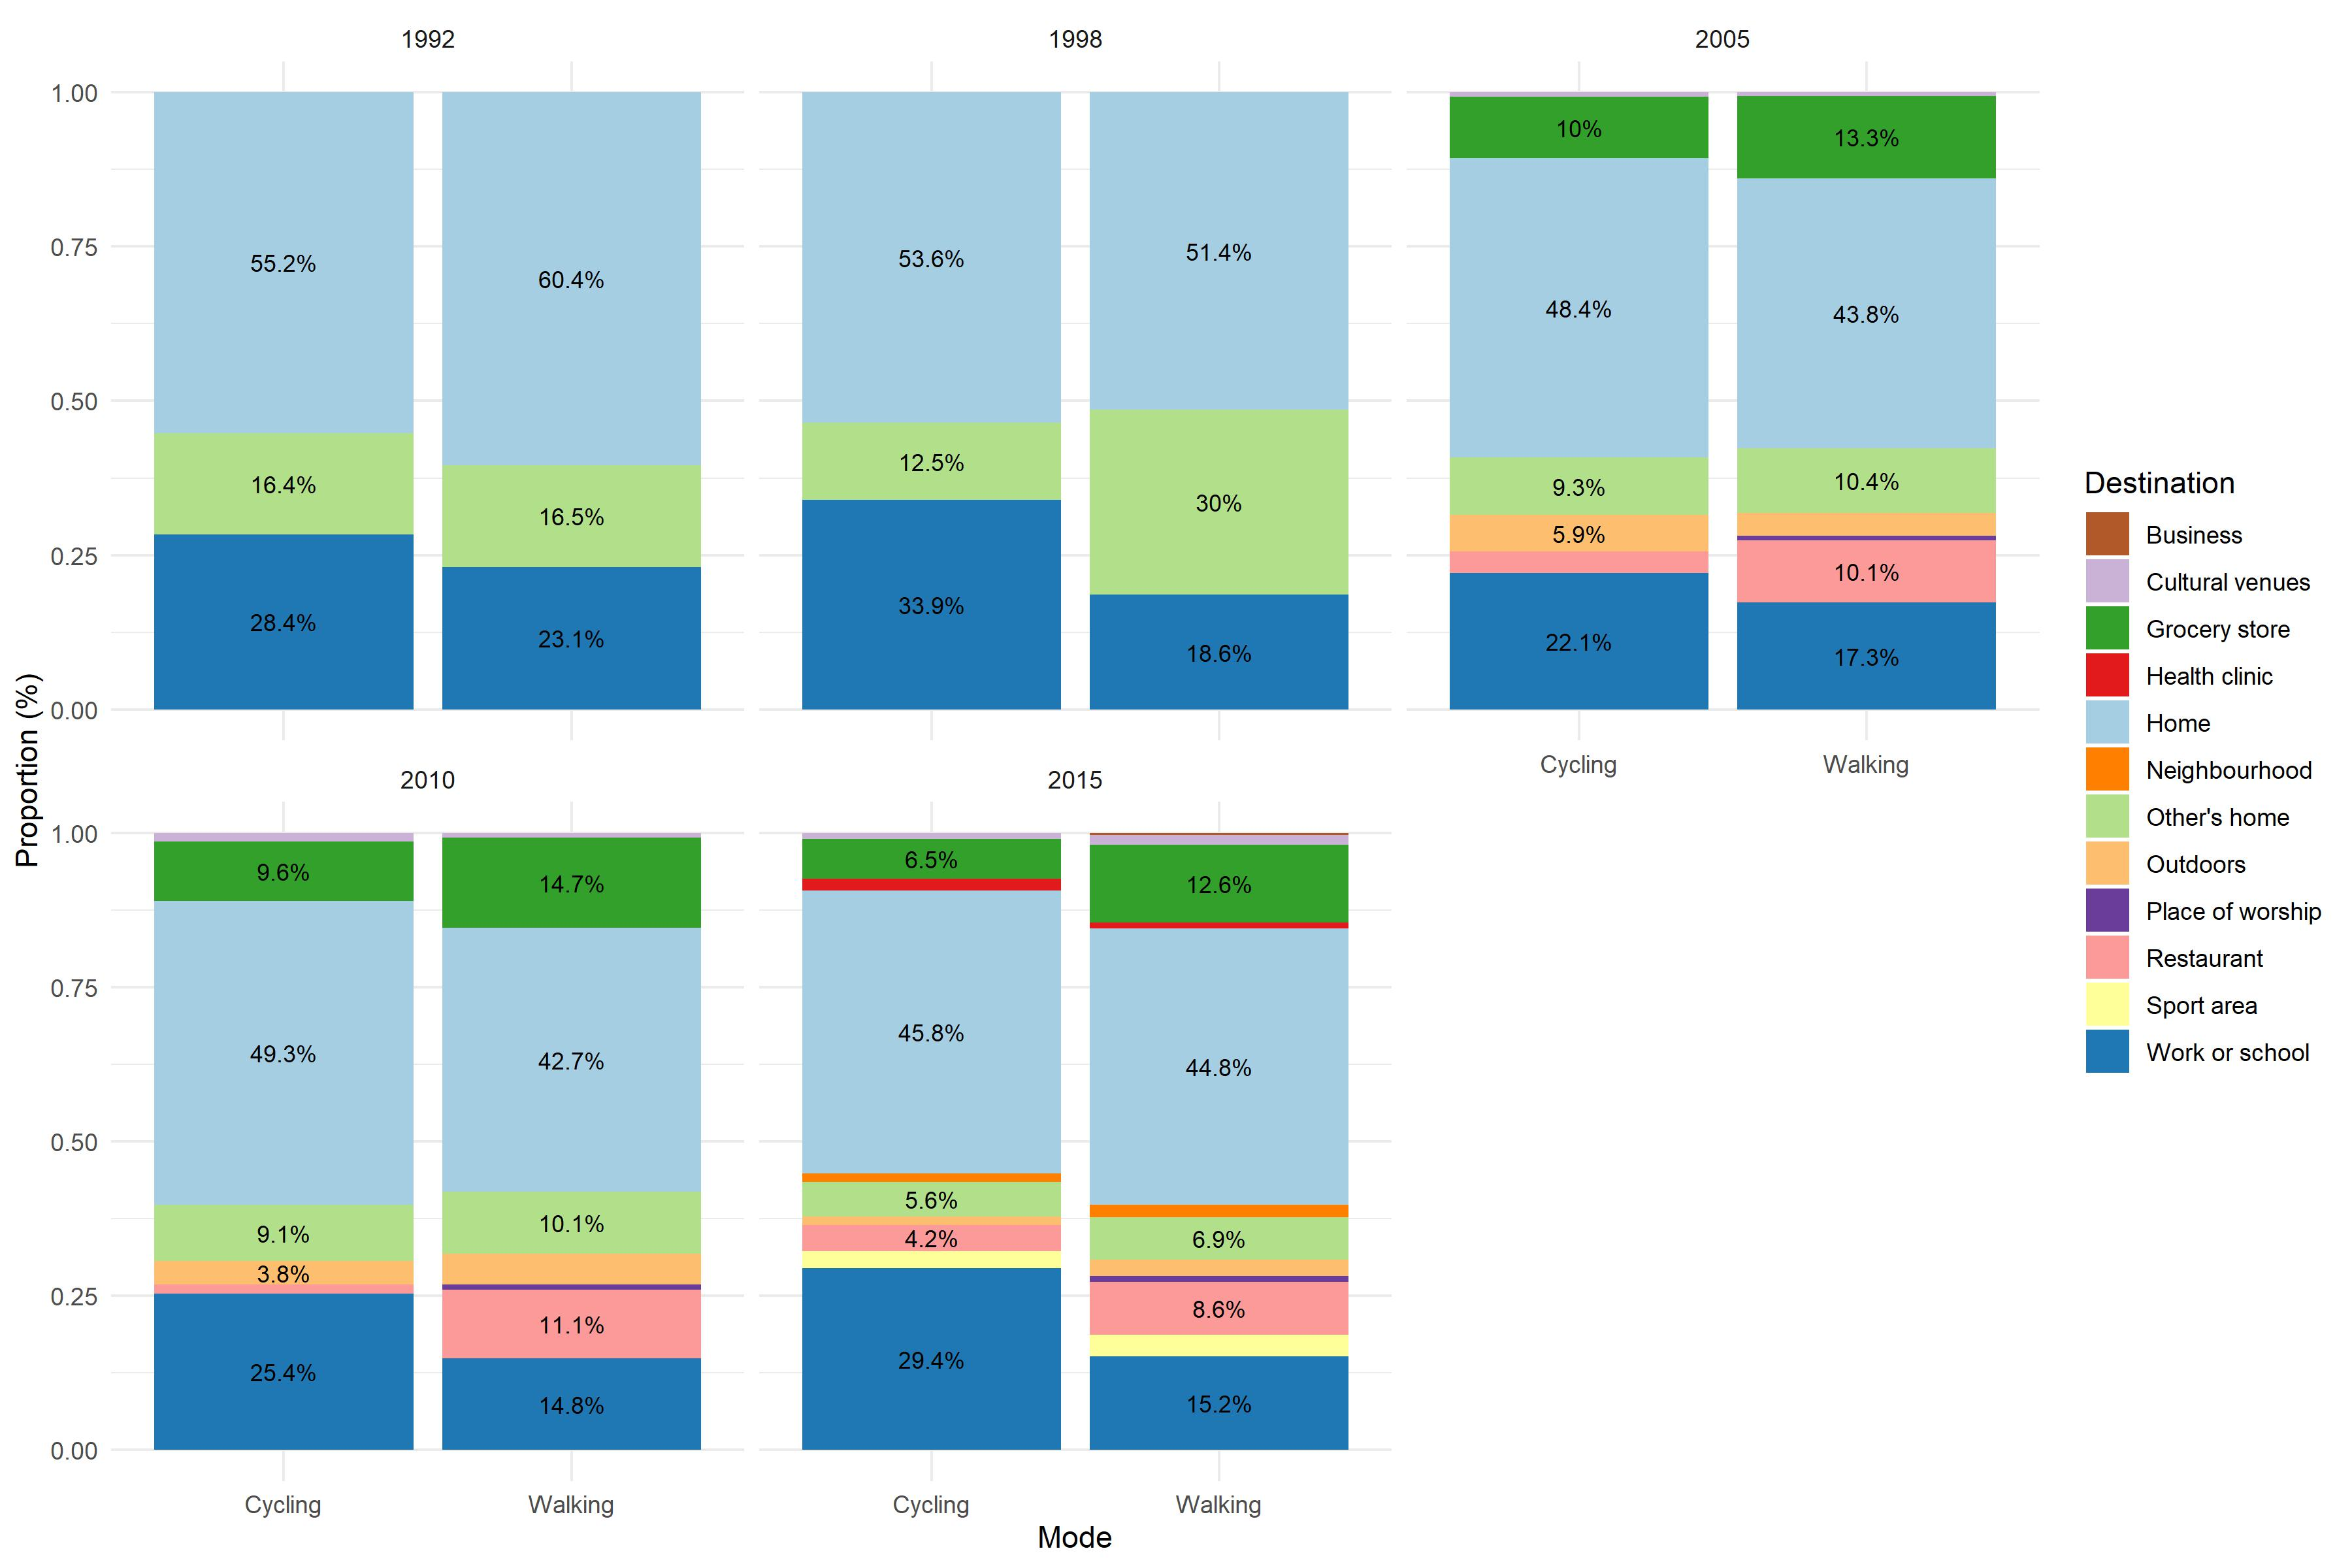
\includegraphics[width=1\linewidth]{figures/destination_percentual} \caption{Percentage of walking and cycling trips categorized by destination and year}\label{fig:figure-destmodeyearperc}
\end{figure}

Figure \ref{fig:figure-boxplot} present the box plot graphs showing the
travel time distribution for active transportation modes over the years,
categorized by destination. Some destinations are presented in only one
survey, such as `Sport area', `Neighbourhood,' and `Business'. These new
destination exhibit typical walking travel times 10 minutes. For cycling
trips, `Business' recorded no trips, while `Sport area' and
`Neighbourhood' registered typical travel times of 30 and 15 minutes,
respectively.

For destinations included in more than one survey, we can compare the
temporal evolution of travel times. Starting with the walking trips, we
can note that there is a tendency of increasing travel times for
`Restaurants' and `Outdoors' (both increasing from 5 in 2005 to 10
minutes in 2015) and `Place of worship' (rising from 10 in 2005 to 15
minutes in 2015). In contrast, some destinations presented a decline in
travel times, where the case of `Cultural venues,' which had a median
travel time of 2005 and drop to 5 minutes in 2015, and `Home' which
start the time series with a minutes in 1992 and dropped to 10 minutes
by 2015. Other destinations maintained an almost constant travel time.
In general, while `Place of worship' displayed the maximum median travel
time of 15 minutes, the general median walking time cuttoff appears to
be 10 minutes, with most of trips occurring below this limit.

For cycling trips, an increasing trend in travel times is evident for
destinations such the destinations `Grocery store' (rising from 10 to 15
minutes between 2005 and 2015), `Outdoors' (increasing from 15 in 2005
to 20 minutes in 2015), and `Home' (retuning to the 1992 typical travel
time of 20 minutes after dropping to 10 minutes in 2010). However,
travel times decreased for destinations like `Other's home' and `Place
of worship', where the typical cycling travel time declined from 20
minutes in their first recorded surveys to 15 minutes by 2015. Other
destinations remained with a constant travel time.

\begin{figure}

\includegraphics[width=1\linewidth]{figures/destination_boxplots} \caption{Percentage of walking trips categorized by origin and destination}\label{fig:figure-boxplot}
\end{figure}

Figures \ref{fig:walking-heatmap} and \ref{fig:cycling-heatmap} show
walking and cycling trips from 1992 to 2015 through heat maps. These
maps use color gradients to represent the percentage of trips between
origins and destinations, with darker colors indicating higher
percentages and lighter colors representing less frequent routes. In
1992, walking trips with `Home' as both the origin and destination made
up the majority, accounting for almost 31\% of all walking trips. These
trips often involved leisure activities, like short walks or dog
walking. Following this, trips from `Home' to `Work or school' comprised
18\% of walking trips. Overall, `Home' is the principal hub, either as
an origin or destination, with only 5\% of trips not involving `Home.'
By 1998, more than half of walking trips were between `Home' and
`Other's home,' with `Home' to `Other's home' and `Other's home' to
`Home' each representing 26\% of trips. During this year, `Home' to
`Home' accounted for only 10\% of trips. In 2005, trips with origins or
destinations involving `Home' and `Work or school' remained as the most
common, but the introduction of new destinations led to a more dispersed
trip distribution. Together, these two combinations accounted for 25\%
of all trips. In 2010, trips between `Home' and `Work or school'
continued as the most common type, representing 18\% of trips, tied with
trips from `Grocery store' to `Home' (9\%). Finishing the walking trip
descriptive analysis, in 2015, the highest proportion of trips were from
`Home' to `Work or school' (12\%) and vice versa (11\%). Trips from
`Home' to `Home' accounted for 8\% of trips, and `Grocery store' became
a notable destination for trips originating from `Home' (8\%).

\begin{figure}
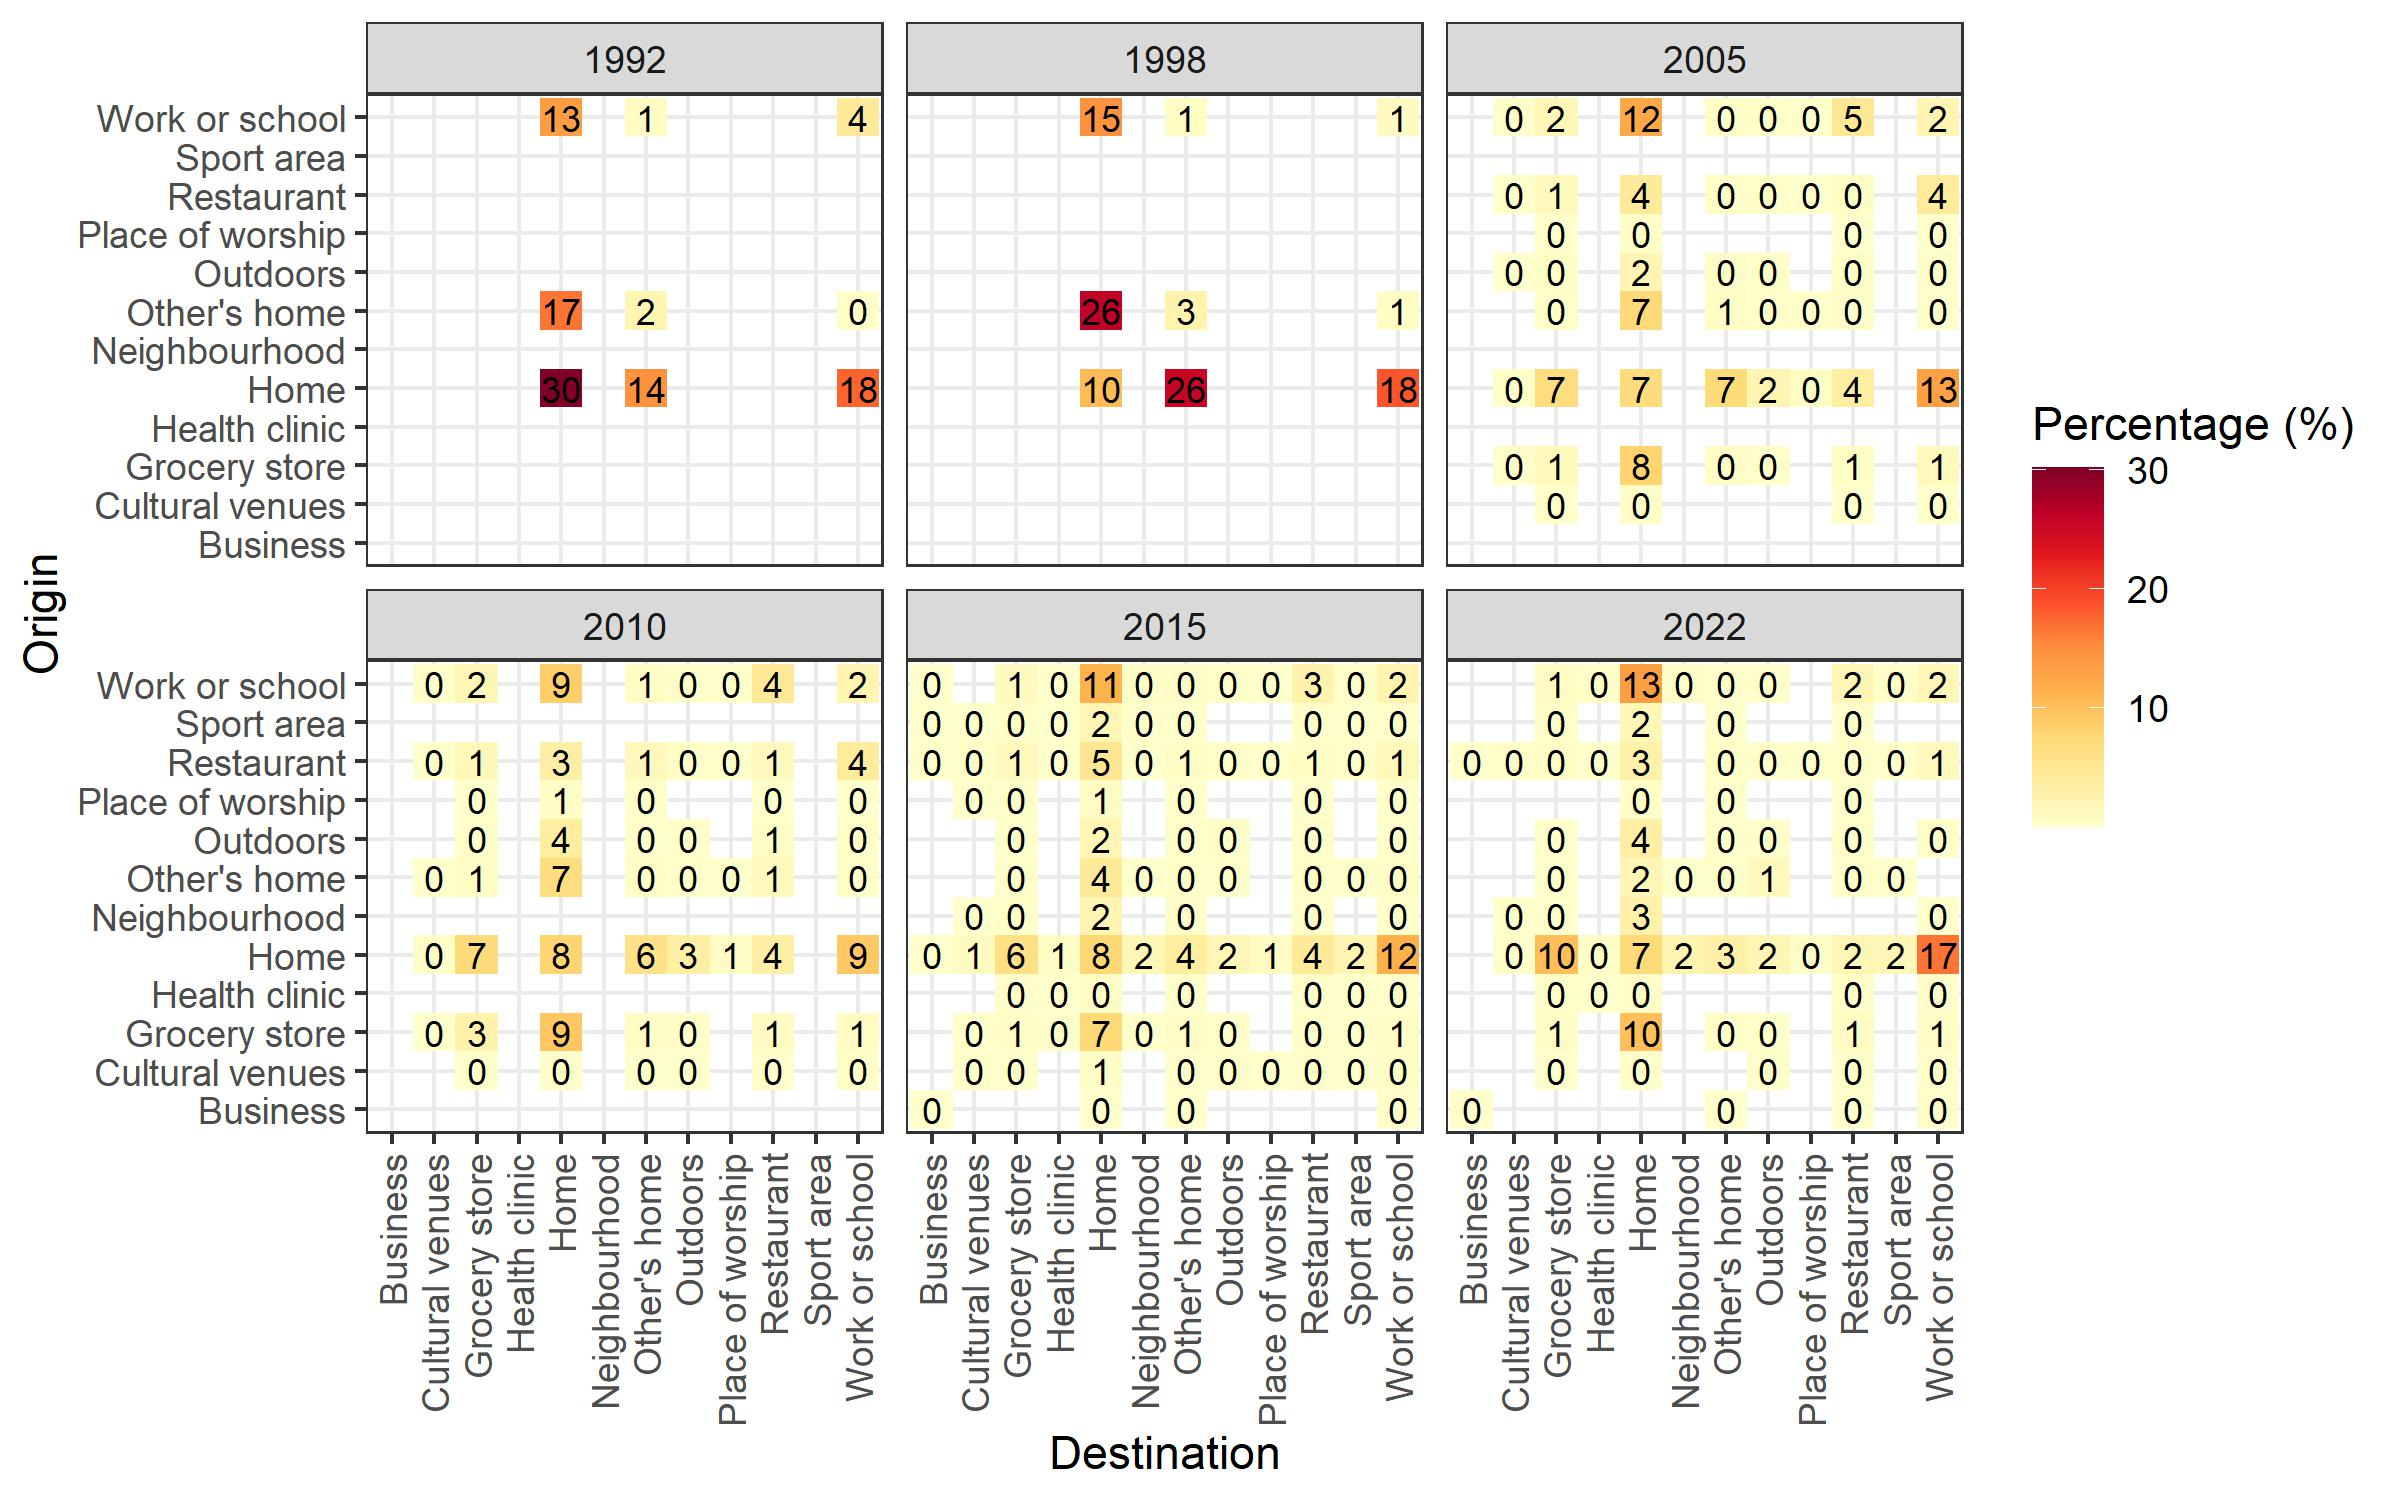
\includegraphics[width=1\linewidth]{figures/walking_hm_fig} \caption{Percentage of walking trips categorized by origin and destination}\label{fig:walking-heatmap}
\end{figure}

For cycling trips (Figure \ref{fig:cycling-heatmap}), in 1992, the most
common trip was from `Home' to `Work or school' (26\%), followed by
trips from `Other's home' to `Home' (22\%). In all following years, the
most frequent trip were between `Home' and `Work or school' in both
direction. This combination accounted for 65\% of the trips in 1998,
40\% in 2005, 52\% in 2010, and 58\% in 2015. Additionally and unlike
walking trips, `Home' to `Home' trips were not a common cycling trip in
any of the surveys. This suggests that leisure trips, such as activities
around the home, are predominantly done by foot rather than by bicycle.

\begin{figure}
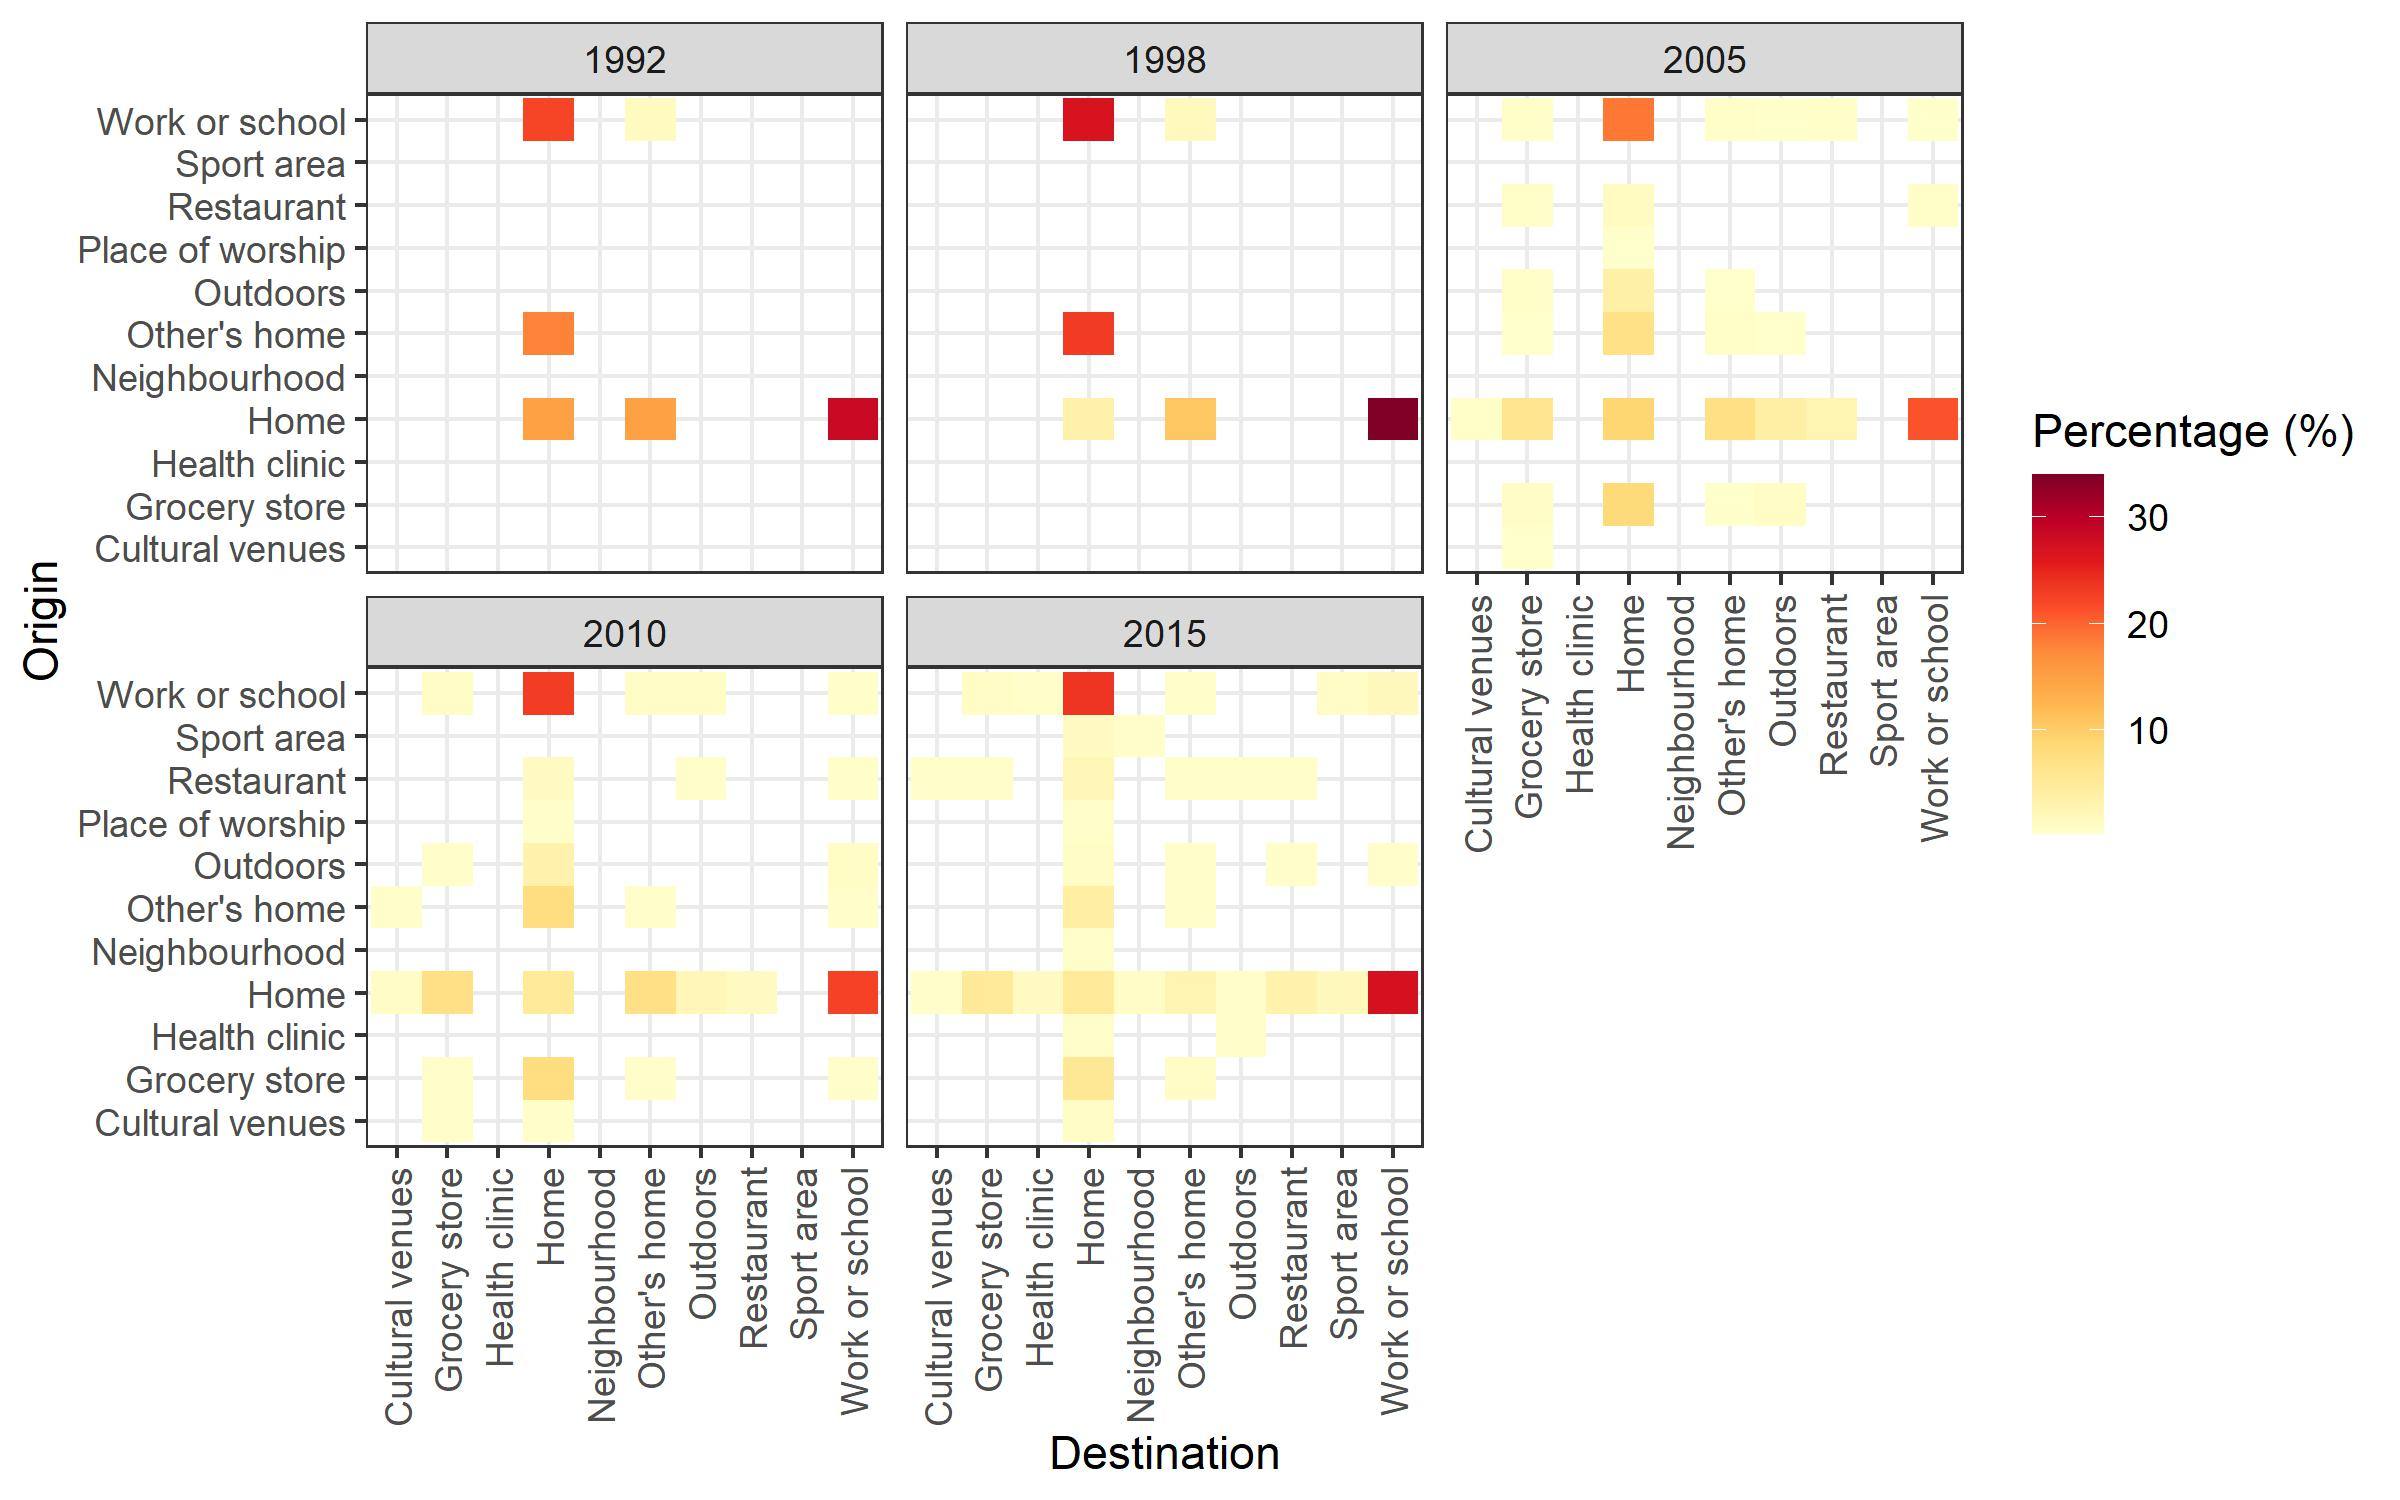
\includegraphics[width=1\linewidth]{figures/cycling_hm_fig} \caption{Percentage of walking trips categorized by origin and destination}\label{fig:cycling-heatmap}
\end{figure}

\hypertarget{calibrated-impedance-function}{%
\subsection{Calibrated impedance
function}\label{calibrated-impedance-function}}

This section presents the identified impedance functions for walking and
cycling trips to various destinations across Canadian Metropolitan and
Census Agglomeration Areas from 1992 to 2015. In general, the impedance
functions aim to capture transportation behavior, illustrating that the
likelihood of traveling between two points decreases as travel duration
increases. Each impedance function follows one of the mathematical
equations previously mentioned, enabling the plotting of PDF curves.
These curves also highlight critical points at which a person's tendency
to walk or cycle significantly decreases.

As explained in the methodology section, we used the \{fitdistrplus\}
package to calibrate the functions. We selected the best impedance
function for each transportation mode, destination, and year based on
the lowest AIC value. The AIC metric not only assesses the goodness of
fit but also penalizes model complexity to prevent overfitting. AIC
provides a balance between a model's accuracy and simplicity, with lower
values indicating a more economical model. The distribution with the
lowest AIC was considered the most suitable for representing the
distance decay curve for each specific destination in each year. We
chose AIC as the selection criterion because, while the \{fitdistrplus\}
package accommodates weighted episodes during estimation, it does not
extend this functionality to diagnostic plots, which are typically
unweighted and traditionally used to select the best-fitting function.

In total, we fitted 64 impedance functions. Among the candidate
distributions, only the lognormal, gamma, and uniform distributions were
selected using our methodology, with the uniform distribution being
chosen exclusively for certain cycling destinations. The absence of
exponential functions, given the variety of destinations, year and mode
of transport, indicates that the impendance functions applied in active
accessibility studies may not be adequately measuring travel behavior.
Table \ref{tab:walking-functions-tab} displays the selected functions
for walking trips, while Table \ref{tab:cycling-functions-table}
presents the functions for cycling trips. Appendix A includes the AIC,
BIC, and log-likelihood values for all candidate distributions.

\begin{table}
\centering
\caption{\label{tab:selected_functions}\label{walking-functions-tab}Impedance functions and AIC for walking trips.}
\centering
\resizebox{\ifdim\width>\linewidth\linewidth\else\width\fi}{!}{
\fontsize{10}{12}\selectfont
\begin{threeparttable}
\begin{tabular}[t]{rllrrrr}
\toprule
\multicolumn{1}{c}{\textbf{Year}} & \multicolumn{1}{c}{\textbf{Destination}} & \multicolumn{1}{c}{\textbf{Impedance function}} & \multicolumn{1}{c}{\textbf{Parameter 1*}} & \multicolumn{1}{c}{\textbf{Parameter 2*}} & \multicolumn{1}{c}{\textbf{AIC}} & \multicolumn{1}{c}{\textbf{Count}}\\
\midrule
1992 & Home & Lognormal & 2.92 & 0.77 & 7761103 & 296\\
1992 & Other's home & Lognormal & 2.15 & 0.84 & 1778150 & 81\\
1992 & Work or school & Lognormal & 2.38 & 0.70 & 2319400 & 113\\
1998 & Home & Lognormal & 2.07 & 0.92 & 5656275 & 302\\
1998 & Other's home & Lognormal & 1.75 & 0.97 & 2892771 & 176\\
\addlinespace
1998 & Work or school & Gamma & 1.23 & 0.09 & 2318752 & 109\\
2005 & Cultural venues & Gamma & 4.10 & 0.34 & 238506 & 25\\
2005 & Grocery store & Gamma & 1.22 & 0.10 & 4776215 & 558\\
2005 & Home & Gamma & 1.16 & 0.08 & 17291041 & 1831\\
2005 & Other's home & Gamma & 1.03 & 0.11 & 3420742 & 436\\
\addlinespace
2005 & Outdoors & Gamma & 1.24 & 0.13 & 1272012 & 155\\
2005 & Place of worship & Gamma & 2.07 & 0.19 & 228307 & 32\\
2005 & Restaurant & Lognormal & 1.95 & 0.79 & 3727576 & 421\\
2005 & Work or school & Lognormal & 2.13 & 0.79 & 8182691 & 724\\
2010 & Cultural venues & Gamma & 3.60 & 0.34 & 304141 & 25\\
\addlinespace
2010 & Grocery store & Lognormal & 2.08 & 0.85 & 6369652 & 489\\
2010 & Home & Gamma & 1.10 & 0.07 & 19584386 & 1424\\
2010 & Other's home & Lognormal & 1.81 & 0.92 & 4035574 & 336\\
2010 & Outdoors & Gamma & 1.27 & 0.13 & 2114346 & 167\\
2010 & Place of worship & Lognormal & 1.95 & 0.70 & 285177 & 28\\
\addlinespace
2010 & Restaurant & Lognormal & 2.01 & 0.90 & 5187191 & 371\\
2010 & Work or school & Lognormal & 2.21 & 0.78 & 7917431 & 494\\
2015 & Business & Lognormal & 2.41 & 0.67 & 102286 & 8\\
2015 & Cultural venues & Gamma & 4.57 & 0.34 & 543242 & 43\\
2015 & Grocery store & Lognormal & 2.48 & 0.68 & 4001111 & 338\\
\addlinespace
2015 & Health clinic & Lognormal & 2.44 & 0.70 & 324578 & 27\\
2015 & Home & Lognormal & 2.57 & 0.74 & 17235960 & 1202\\
2015 & Neighbourhood & Lognormal & 2.41 & 0.77 & 981626 & 53\\
2015 & Other's home & Lognormal & 2.43 & 0.80 & 2388598 & 186\\
2015 & Outdoors & Lognormal & 2.54 & 0.79 & 1247963 & 72\\
\addlinespace
2015 & Place of worship & Gamma & 5.64 & 0.28 & 343187 & 24\\
2015 & Restaurant & Lognormal & 2.38 & 0.74 & 3490082 & 231\\
2015 & Sport area & Lognormal & 2.48 & 0.59 & 1199687 & 94\\
2015 & Work or school & Lognormal & 2.55 & 0.64 & 6612061 & 407\\
\bottomrule
\end{tabular}
\begin{tablenotes}
\item \textit{Note: } 
\item For 'lnorm' distributions, 'Parameter 1' and 'Parameter 2' refer to the mean and standard deviation of the distribution on the logarithmic scaler, respectively. For the 'Gamma' distribution, 'Parameter 1' and 'Parameter 2' refer to the rate and shape of the distribution, respectively. For the 'Uniform' distribution,  'Parameter 1' refers to the minimum lower bound and 'Parameter 2'  refers to the upper bound (maximum) of the distribution.  'AIC' means Akaike information criterion.
\end{tablenotes}
\end{threeparttable}}
\end{table}

\begin{table}
\centering
\caption{\label{tab:selected_functions}\label{cycling-functions-tab}Impedance functions and AIC for cycling trips.}
\centering
\resizebox{\ifdim\width>\linewidth\linewidth\else\width\fi}{!}{
\fontsize{10}{12}\selectfont
\begin{threeparttable}
\begin{tabular}[t]{rllrrrr}
\toprule
\multicolumn{1}{c}{\textbf{Year}} & \multicolumn{1}{c}{\textbf{Destination}} & \multicolumn{1}{c}{\textbf{Impedance function}} & \multicolumn{1}{c}{\textbf{Parameter 1*}} & \multicolumn{1}{c}{\textbf{Parameter 2*}} & \multicolumn{1}{c}{\textbf{AIC}} & \multicolumn{1}{c}{\textbf{Count}}\\
\midrule
1992 & Home & Gamma & 1.18 & 0.05 & 1018747 & 37\\
1992 & Other's home & Lognormal & 2.57 & 0.82 & 373451 & 11\\
1992 & Work or school & Gamma & 3.00 & 0.17 & 433582 & 19\\
1998 & Home & Gamma & 1.70 & 0.07 & 715802 & 30\\
1998 & Other's home & Lognormal & 2.79 & 0.80 & 113905 & 7\\
\addlinespace
1998 & Work or school & Gamma & 3.37 & 0.10 & 481536 & 19\\
2005 & Cultural venues & Uniform & 0.00 & 15.13 & 6355 & 2\\
2005 & Grocery store & Gamma & 1.93 & 0.14 & 320218 & 29\\
2005 & Home & Gamma & 1.49 & 0.07 & 1794317 & 140\\
2005 & Other's home & Gamma & 1.84 & 0.15 & 310058 & 27\\
\addlinespace
2005 & Outdoors & Gamma & 2.99 & 0.17 & 215894 & 17\\
2005 & Restaurant & Gamma & 3.37 & 0.21 & 109072 & 10\\
2005 & Work or school & Lognormal & 2.93 & 0.70 & 888655 & 64\\
2010 & Cultural venues & Uniform & 0.00 & 32.58 & 38938 & 3\\
2010 & Grocery store & Lognormal & 2.68 & 0.61 & 315037 & 20\\
\addlinespace
2010 & Home & Lognormal & 2.60 & 0.77 & 2006242 & 103\\
2010 & Other's home & Lognormal & 2.40 & 0.63 & 338777 & 19\\
2010 & Outdoors & Lognormal & 2.05 & 0.59 & 92699 & 8\\
2010 & Restaurant & Uniform & 0.00 & 17.49 & 35370 & 3\\
2010 & Work or school & Lognormal & 2.65 & 0.77 & 1292760 & 53\\
\addlinespace
2015 & Cultural venues & Lognormal & 2.71 & 0.00 & -Inf & 2\\
2015 & Grocery store & Lognormal & 3.08 & 0.80 & 229413 & 14\\
2015 & Health clinic & Lognormal & 2.93 & 0.86 & 80810 & 4\\
2015 & Home & Lognormal & 3.08 & 0.61 & 1745846 & 98\\
2015 & Neighbourhood & Uniform & 0.00 & 48.55 & 49924 & 3\\
\addlinespace
2015 & Other's home & Lognormal & 2.52 & 0.44 & 140210 & 12\\
2015 & Outdoors & Uniform & 0.00 & 35.03 & 31463 & 3\\
2015 & Restaurant & Lognormal & 3.11 & 0.60 & 115406 & 9\\
2015 & Sport area & Uniform & 0.00 & 17.47 & 32969 & 6\\
2015 & Work or school & Lognormal & 3.03 & 0.41 & 1162876 & 63\\
\bottomrule
\end{tabular}
\begin{tablenotes}
\item \textit{Note: } 
\item For 'lnorm' distributions, 'Parameter 1' and 'Parameter 2' refer to the mean and standard deviation of the distribution on the logarithmic scaler, respectively. For the 'Gamma' distribution, 'Parameter 1' and 'Parameter 2' refer to the rate and shape of the distribution, respectively. For the 'Uniform' distribution,  'Parameter 1' refers to the minimum lower bound and 'Parameter 2'  refers to the upper bound (maximum) of the distribution.  'AIC' means Akaike information criterion.
\end{tablenotes}
\end{threeparttable}}
\end{table}

Figure X presents the calibrated functions for the destination
``Outdoors,'' along with a histogram of the empirical distribution of
trips, split by year and transportation mode. Comparing functions from
different categories can be tricky when analyzed for the first time, but
by starting with the functions from the walking transportation mode, the
calibrated functions from this example show a similar pattern. At a
duration of around zero minutes, the probability of making the trip is
low (with a density of zero for the years 2010 and 2015). After a few
minutes, there is a peak in the maximum probability of traveling to
reach ``Outdoors,'' followed by a drop in willingness to zero for very
high values of time, indicating a low probability of making the trip.

For the years 2005 and 2010, the selected impedance functions are of the
gamma type, with shapes of \(\alpha = 1.24\) and \(\alpha = 1.27\),
respectively, and the same rate of \(\sigma = 0.13\). The rate parameter
(\(\sigma\)) mainly controls the speed of the curved drop, which is the
same for both years. The shape parameter (\(\mu\)) controls how the
density peak shifts in relation to the \(x\)-axis (the travel time). A
larger shape value means that the probability peak occurs at larger
values of time. Since the shape values for 2005 and 2010 are very close,
the peak of the PDF curve in both cases occurs at 2 minutes. Although
the difference in shape (\(\mu\)) between the two years is small and
does not change the time at which the peak occurs, it is enough to cause
a difference in the peak values themselves. In 2005, the walking trips
had a higher density around 2 minutes (0.079) compared to 2010 (0.077).

For 2015, the PDF that best represents the population's transport
behavior is a lognormal distribution, with a mean of \(\mu = 3.08\) and
a standard deviation of \(\sigma = 0.80\). In this year, the density
peak (0.05) occurs when the journey has the duration of 7 minutes. Here,
we can see that a lower density peak also corresponds to a more
dispersed curve, with higher densities at larger values of time. In
fact, while in 2005 and 2010 walking trips had densities close to zero
for values over 50 minutes, in 2015 there is still a small density
(0.002) at the 50-minute mark.

For trips made by bicycle, in 2015 and 2010 the impedance functions are
of the gamma type, with a shape of \(\alpha = 2.99\) and
\(\alpha = 2.05\), respectively, and rates \(\sigma = 0.17\) and
\(\sigma = 0.59\). Such configurations in the gamma function result in
different peak values, where in 2005 the peak (0.046) of density
occurred in 12 minutes, in 2010 the peak (0.102) occurs in 6 minutes,
half the previous time. In 2005, the curve has a smaller peak and is
more dispersed, while in 2010 the curve has a larger peak and is less
dispersed, reinforced by its higher \(\sigma\) rate.

In 2005, the PDF that best represented the curve was a uniform function
with upper bound equals to 35 minutes and peak of (0.028). The presence
of uniform functions means that it wasn't possible to parameterize more
complex functions (like the other functions) and is explained by the low
number of episodes in this category of destination, mode of transport
and year (in this case, there were only 3 episodes identified). Overall,
all the uniform functions have a maximum of 6 episodes and all of them
are for the transportation mode cycling - which can be explained since
this mode of transport doesn't have many episodes compared to the
walking episodes. The figure also shows how cycling trips tend to have
greater dispersion and higher typical values (dashed vertical lines)
when compared to walking trips.

\begin{figure}

{\centering 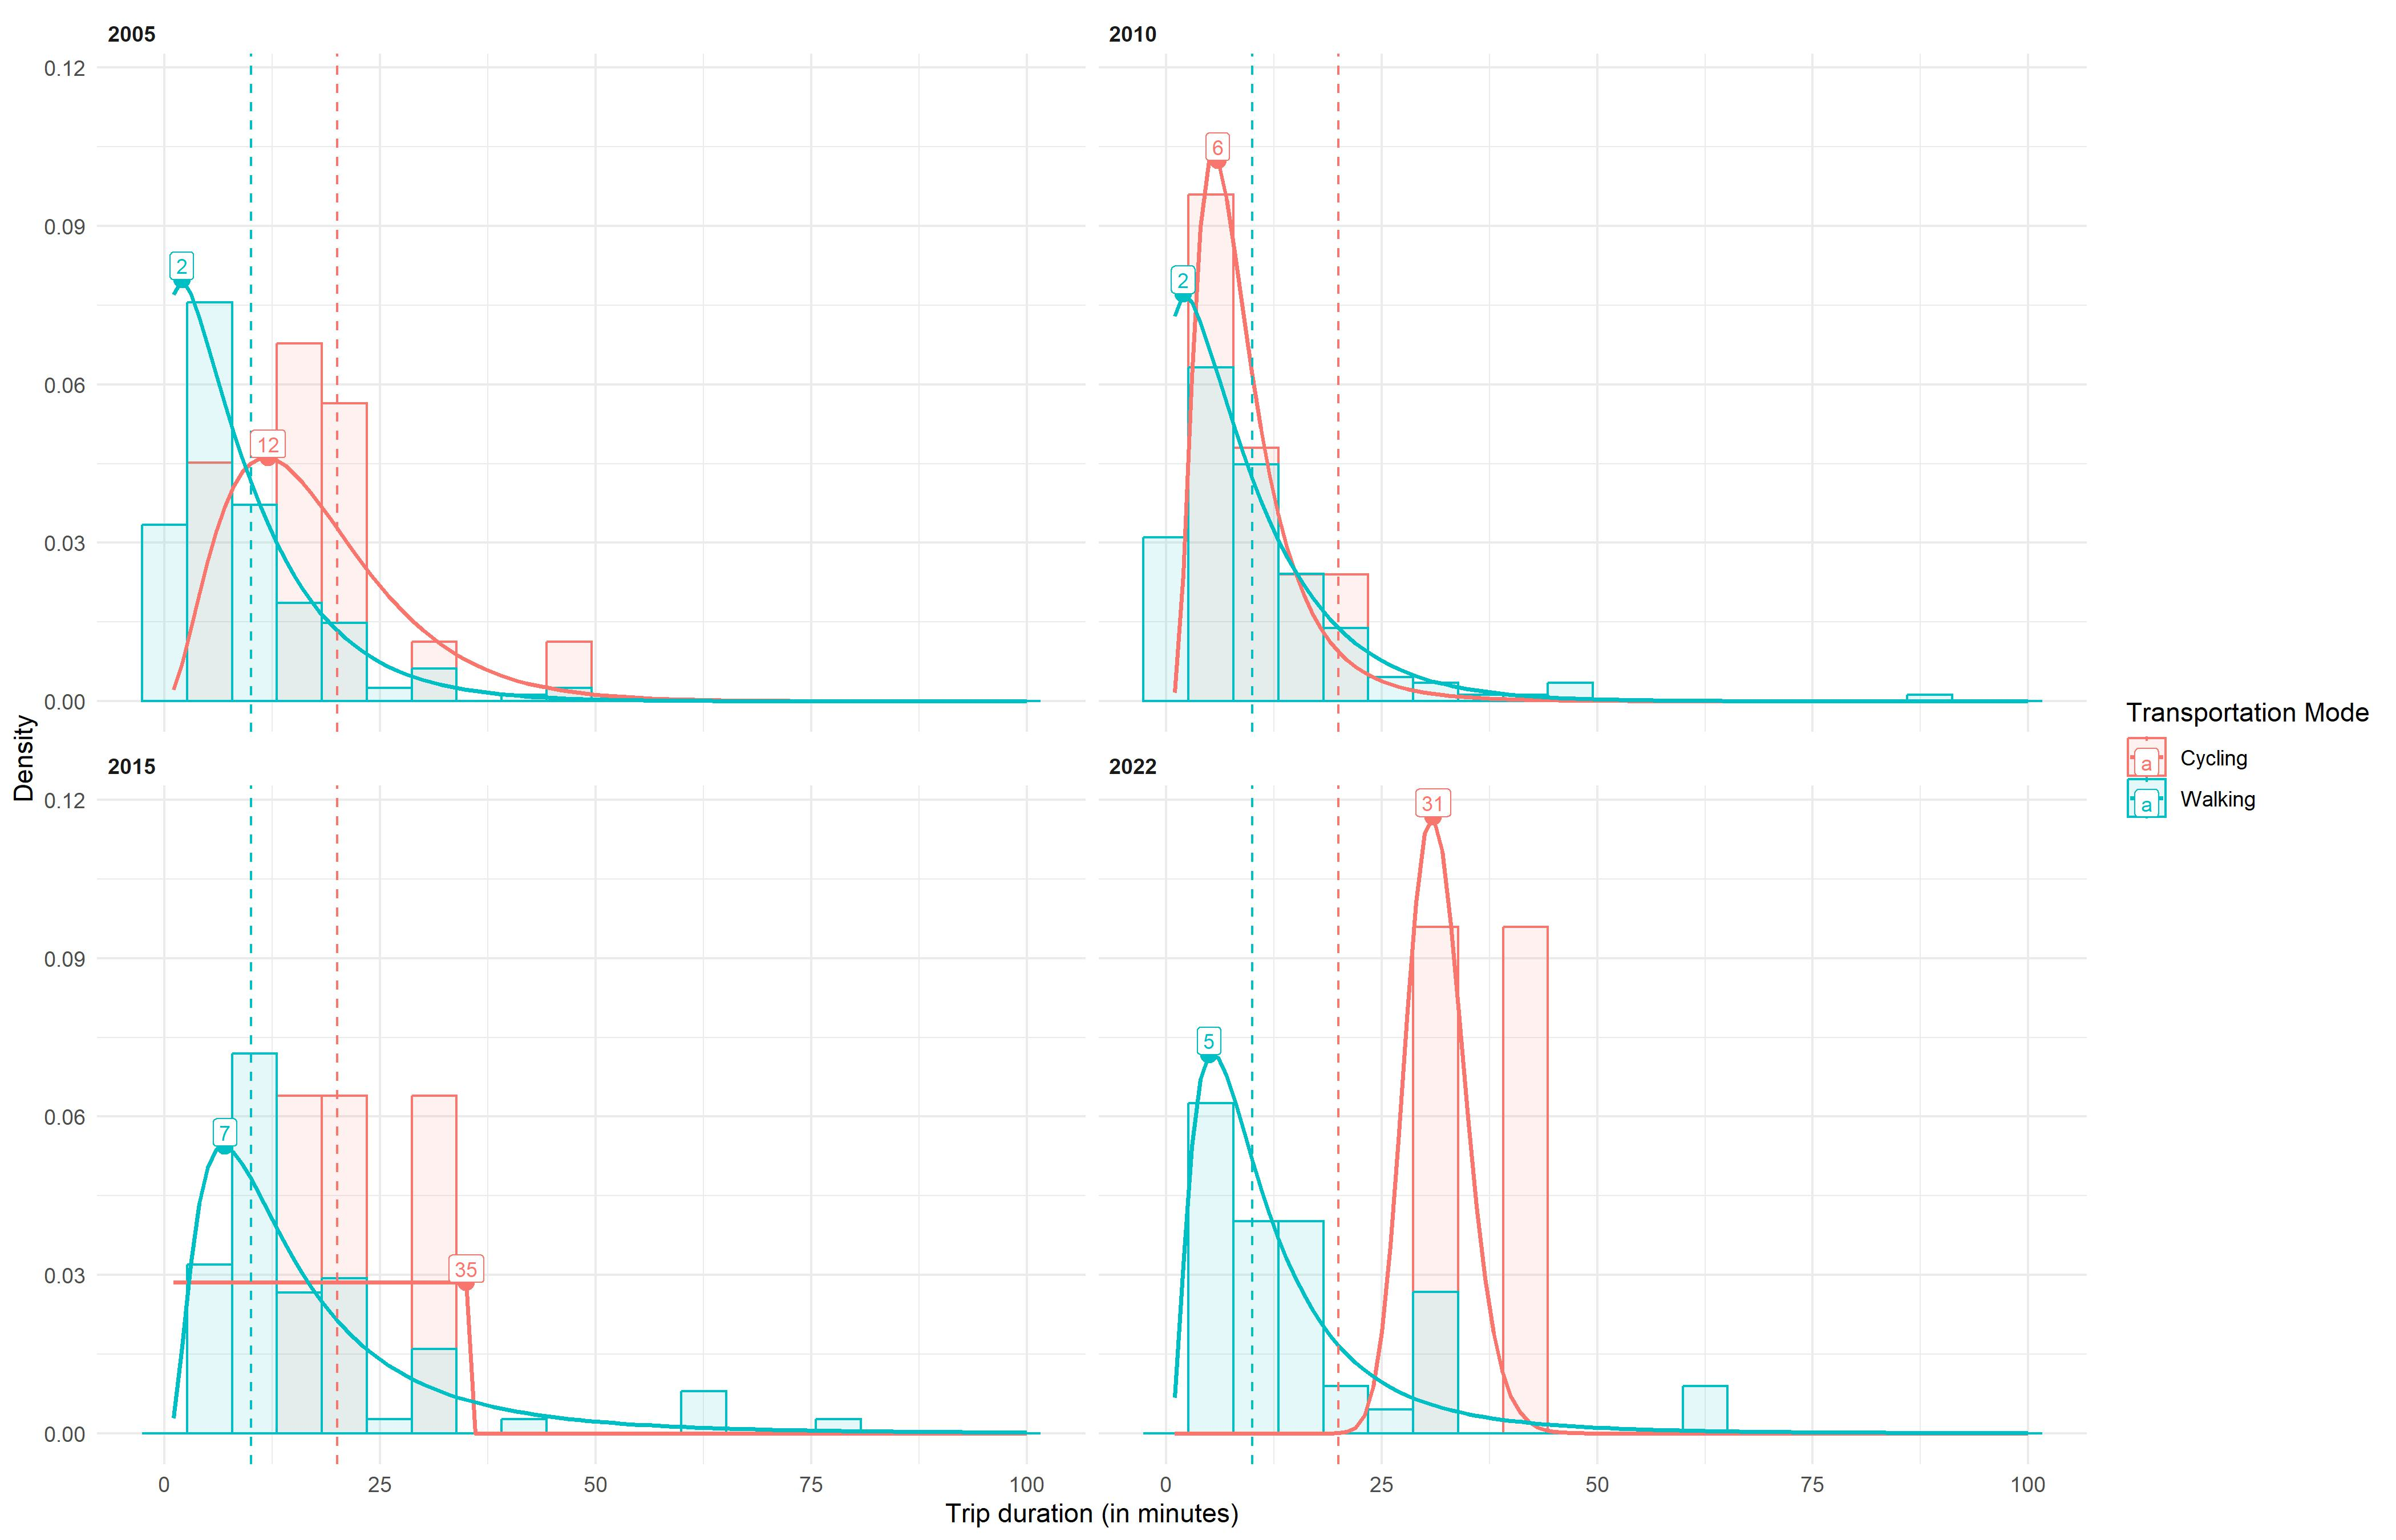
\includegraphics[width=1\linewidth]{figures/impf_Outdoors} 

}

\caption{Empirical data and impedance functions fitted for walking trips with `work or school` as destination.}\label{fig:outdoors-impedance-fig}
\end{figure}

This temporal difference between the decay functions is also evident in
Figure (temp-evolution-by-destination), which shows the calibrated
functions for each year of analysis across all destination and transport
mode categories for walking trips. For some locations, the impedance
functions are of the same type and have similar parameters across all
the years analyzed. For example, the ``Cultural venues'' destination
consistently uses a gamma function to represent the population's
transport behavior for all the years analyzed. On the other hand, the
``Place of worship'' destination exhibits temporal differences, with
distinctly different peaks and density dispersions, reflecting the
variations in the empirical data shown in Figure
\ref{fig:figure-boxplot} and discussed above.

\begin{figure}

{\centering 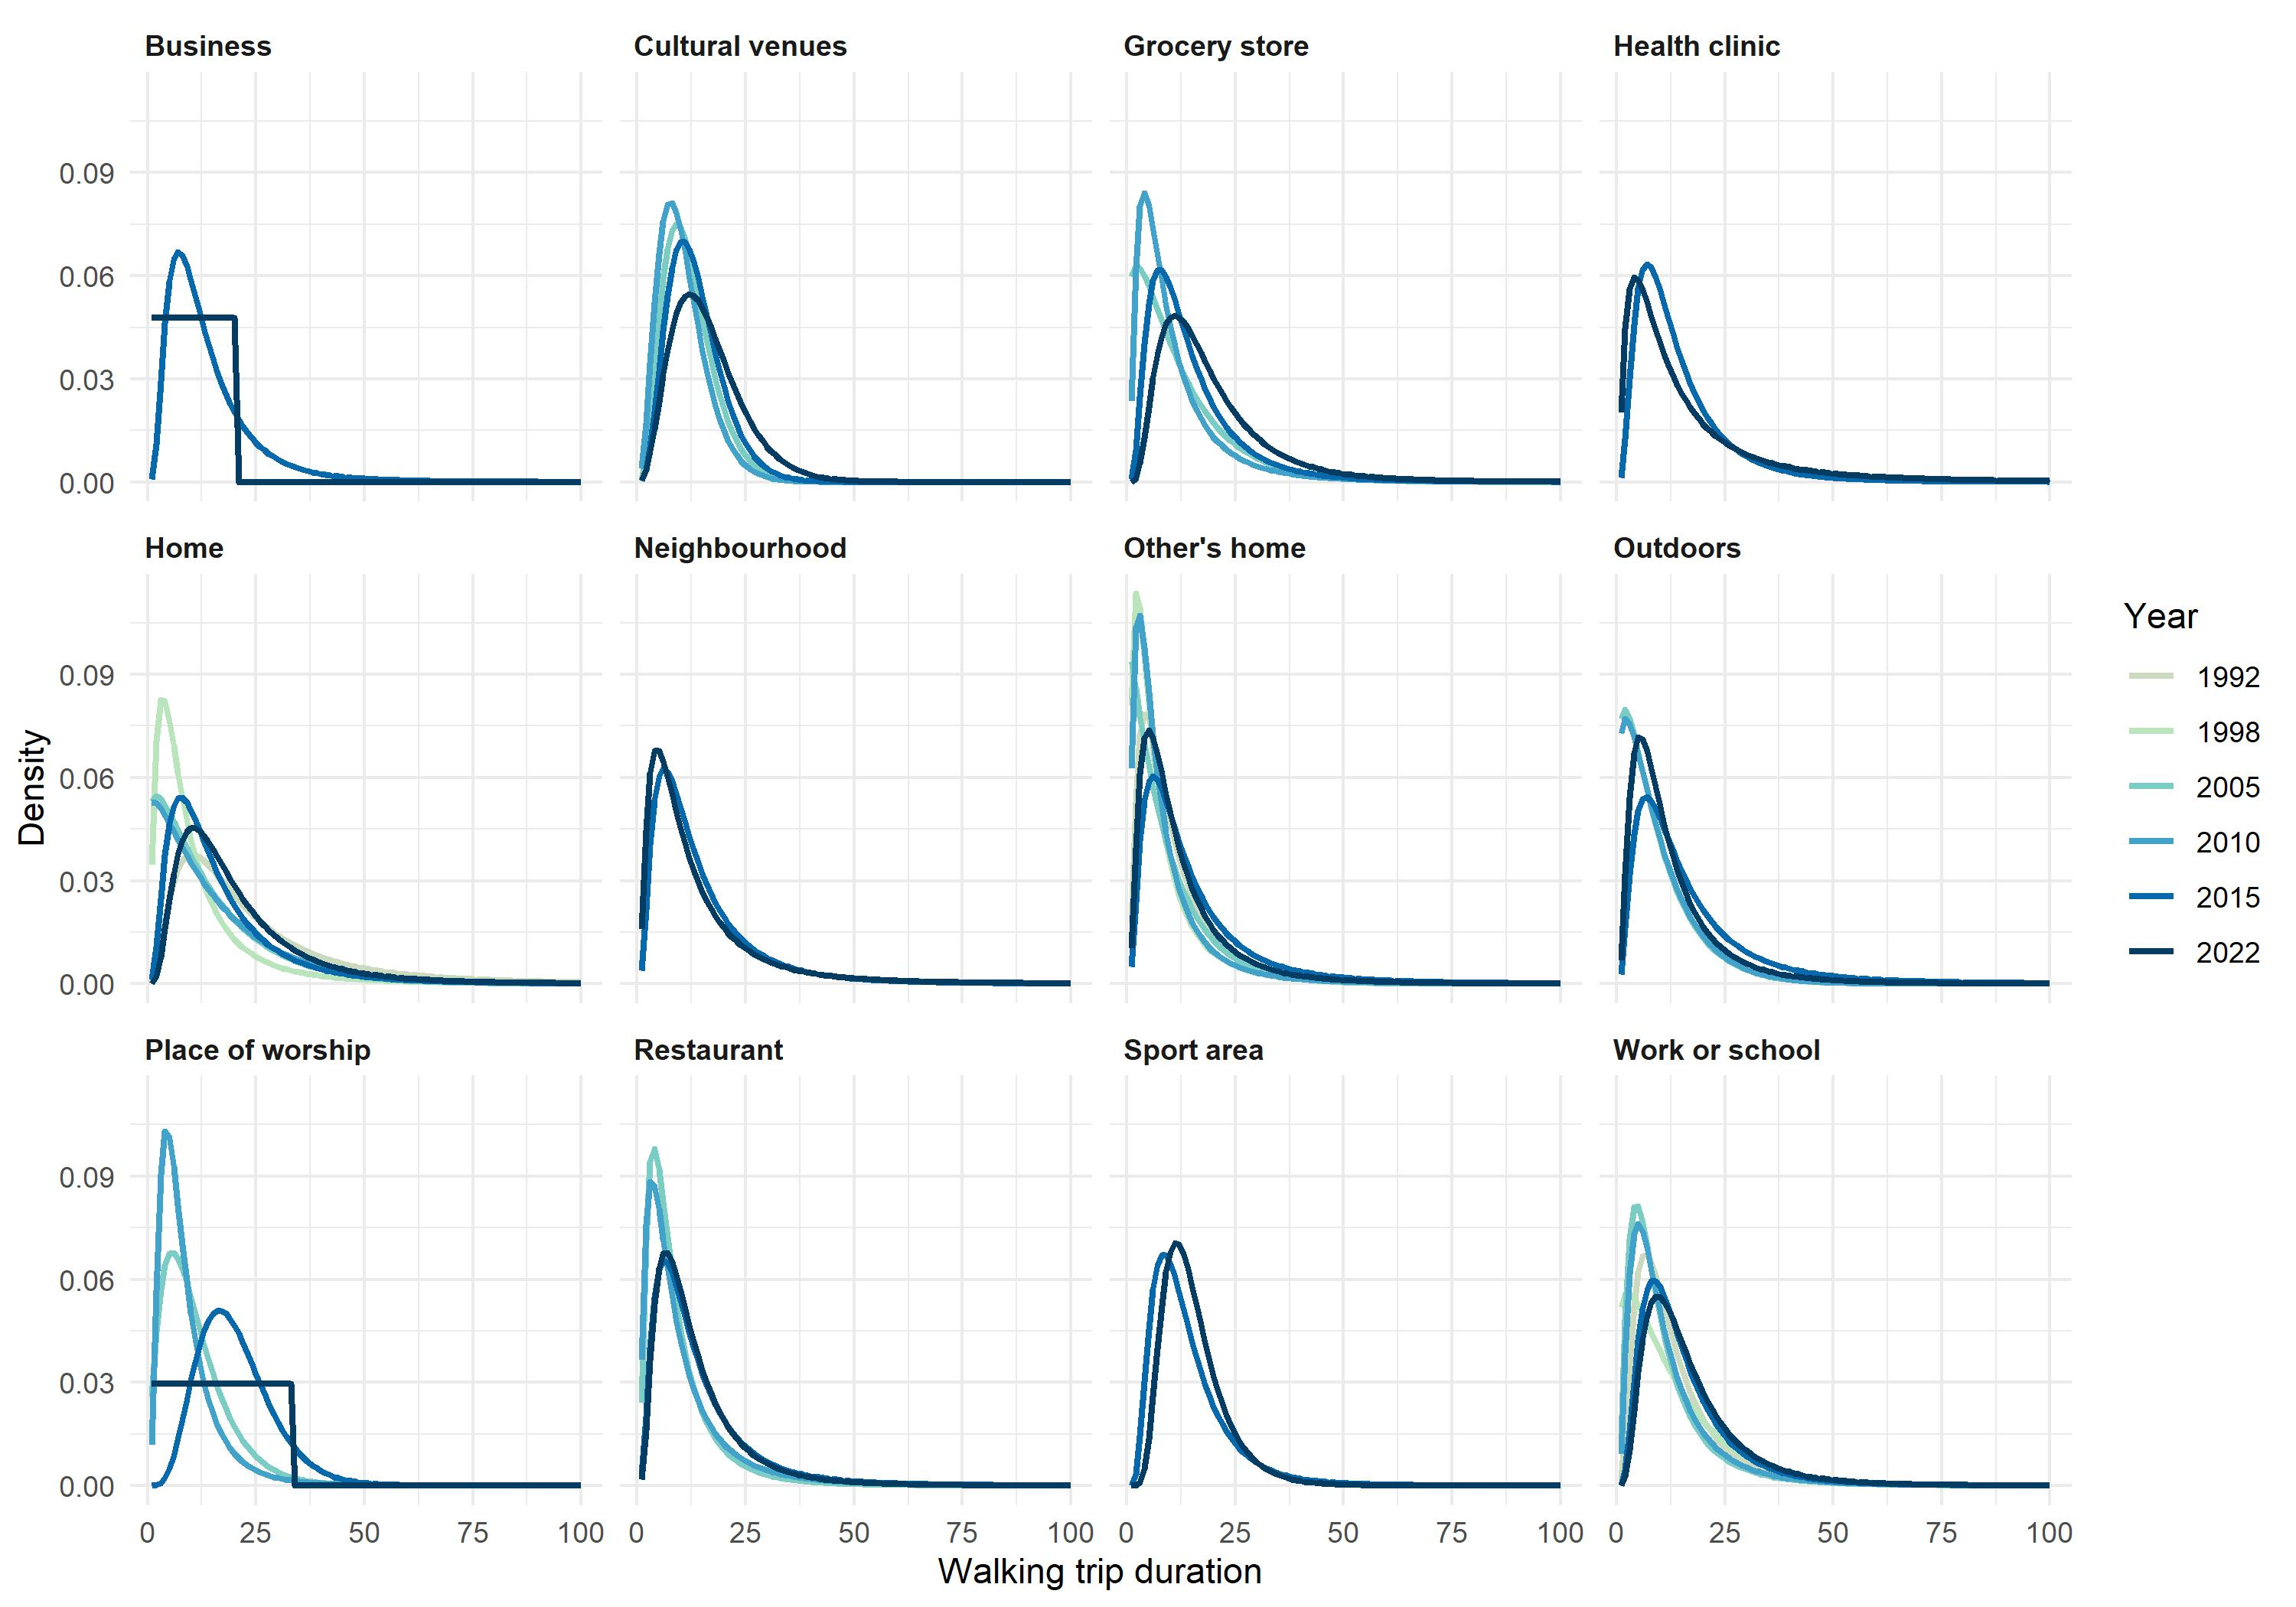
\includegraphics[width=1\linewidth]{figures/walking_temporal_evolution} 

}

\caption{Temporal evolution of walking impedance functions.}\label{fig:walking-evolution-fig}
\end{figure}

Only destinations that appear in more than one year can have their
temporal evolution analyzed. Because of this, for the twelve possible
destinations in the cycling mode, only seven locations can be temporally
analyzed: ``Cultural venues,'' ``Grocery store,'' ``Home,'' ``Other's
home,'' ``Outdoors,'' ``Restaurant,'' and ``Work or school.'' In the
case of the walking trips, this transporation mode is present in more
than one survey for the same locations as cycling mode, as well as for
``Place of worship.''

After performing the Kruskal-Wallis test (to assess whether there was a
statistically significant difference between the distributions of
empirical travel time values, considering the time differences for each
destination) and the pairwise Wilcoxon test, we were able to identify
the destinations where a statistically significant difference was
detected. Table \ref{tab:result-stats} shows only the destinations where
a statistically significant difference was found, considering the two
modes of active transport analyzed.

For cycling trips, the destinations ``Home,'' ``Grocery store,''
``Restaurant,'' and ``Work or school'' had at least one year with a
statistically significant difference. For example, for the ``Home''
destination, there was a statistically significant difference between
1992 and 2005 (p-value = 0.0046), 1992 and 2010 (p-value = 0.0003), 1998
and 2005 (p-value = 0.0390), 1998 and 2010 (p-value = 0.0412), 1998 and
2015 (p-value = 0.0196), 2005 and 2010 (p-value = 0.00017), and 2010 and
2015 (p-value = 0.01008).

For walking trips, among the destinations with a potential time
difference, only ``Cultural venues'' did not show a statistically
significant difference during the period analyzed. As a result, among
the destinations appearing in more than one GSS survey, only ``Cultural
venues'' showed no statistical evidence of temporal evolution for any of
the modes of transport. Four destinations (``Home,'' ``Grocery store,''
``Restaurant,'' and ``Work or school'') exhibited statistical
differences for both modes of transport.

\begin{table}
\centering
\caption{\label{tab:stats-table}\label{result-stats}P-values of the pairwise Wilcoxon test .}
\centering
\resizebox{\ifdim\width>\linewidth\linewidth\else\width\fi}{!}{
\fontsize{10}{12}\selectfont
\begin{tabular}[t]{lllrrrr}
\toprule
Mode & Destination & Year & 1992 & 1998 & 2005 & 2010\\
\midrule
Walking & Restaurant & 2010 & NA & NA & 0.00003 & NA\\
Walking & Restaurant & 2015 & NA & NA & 0.00003 & 0.00001\\
Walking & Grocery store & 2010 & NA & NA & 0.00000 & NA\\
Walking & Grocery store & 2015 & NA & NA & NA & 0.00159\\
Walking & Home & 1998 & 0.00000 & NA & NA & NA\\
\addlinespace
Walking & Home & 2005 & 0.00000 & 0.00000 & NA & NA\\
Walking & Home & 2010 & 0.00000 & 0.00000 & 0.00000 & NA\\
Walking & Home & 2015 & 0.00000 & 0.00000 & 0.00000 & NA\\
Walking & Work or school & 1998 & 0.00871 & NA & NA & NA\\
Walking & Work or school & 2015 & NA & 0.00004 & 0.00483 & NA\\
\addlinespace
Walking & Other's home & 1998 & 0.00000 & NA & NA & NA\\
Walking & Other's home & 2010 & 0.00003 & 0.01048 & 0.04166 & NA\\
Walking & Other's home & 2015 & NA & 0.00000 & 0.00000 & 0.00000\\
Walking & Place of worship & 2015 & NA & NA & 0.01946 & NA\\
Walking & Outdoors & 2015 & NA & NA & 0.00000 & 0.00044\\
\addlinespace
Cycling & Restaurant & 2010 & NA & NA & 0.03883 & NA\\
Cycling & Restaurant & 2015 & NA & NA & NA & 0.04323\\
Cycling & Home & 2005 & 0.00460 & 0.03902 & NA & NA\\
Cycling & Home & 2010 & 0.00030 & 0.04117 & 0.00017 & NA\\
Cycling & Home & 2015 & NA & 0.01960 & NA & 0.01008\\
\addlinespace
Cycling & Work or school & 1998 & 0.02112 & NA & NA & NA\\
Cycling & Work or school & 2005 & NA & 0.03558 & NA & NA\\
Cycling & Work or school & 2015 & NA & 0.00190 & 0.00242 & 0.00290\\
Cycling & Grocery store & 2015 & NA & NA & 0.00278 & NA\\
\bottomrule
\end{tabular}}
\end{table}

Finally, Figures \ref{fig:walking-function-by-year-fig} and
\ref{fig:cycling-function-by-year-fig} present the impedance functions
for different destination categories, grouped by year, for the walking
and cycling modes of transport, respectively.

\begin{figure}

{\centering 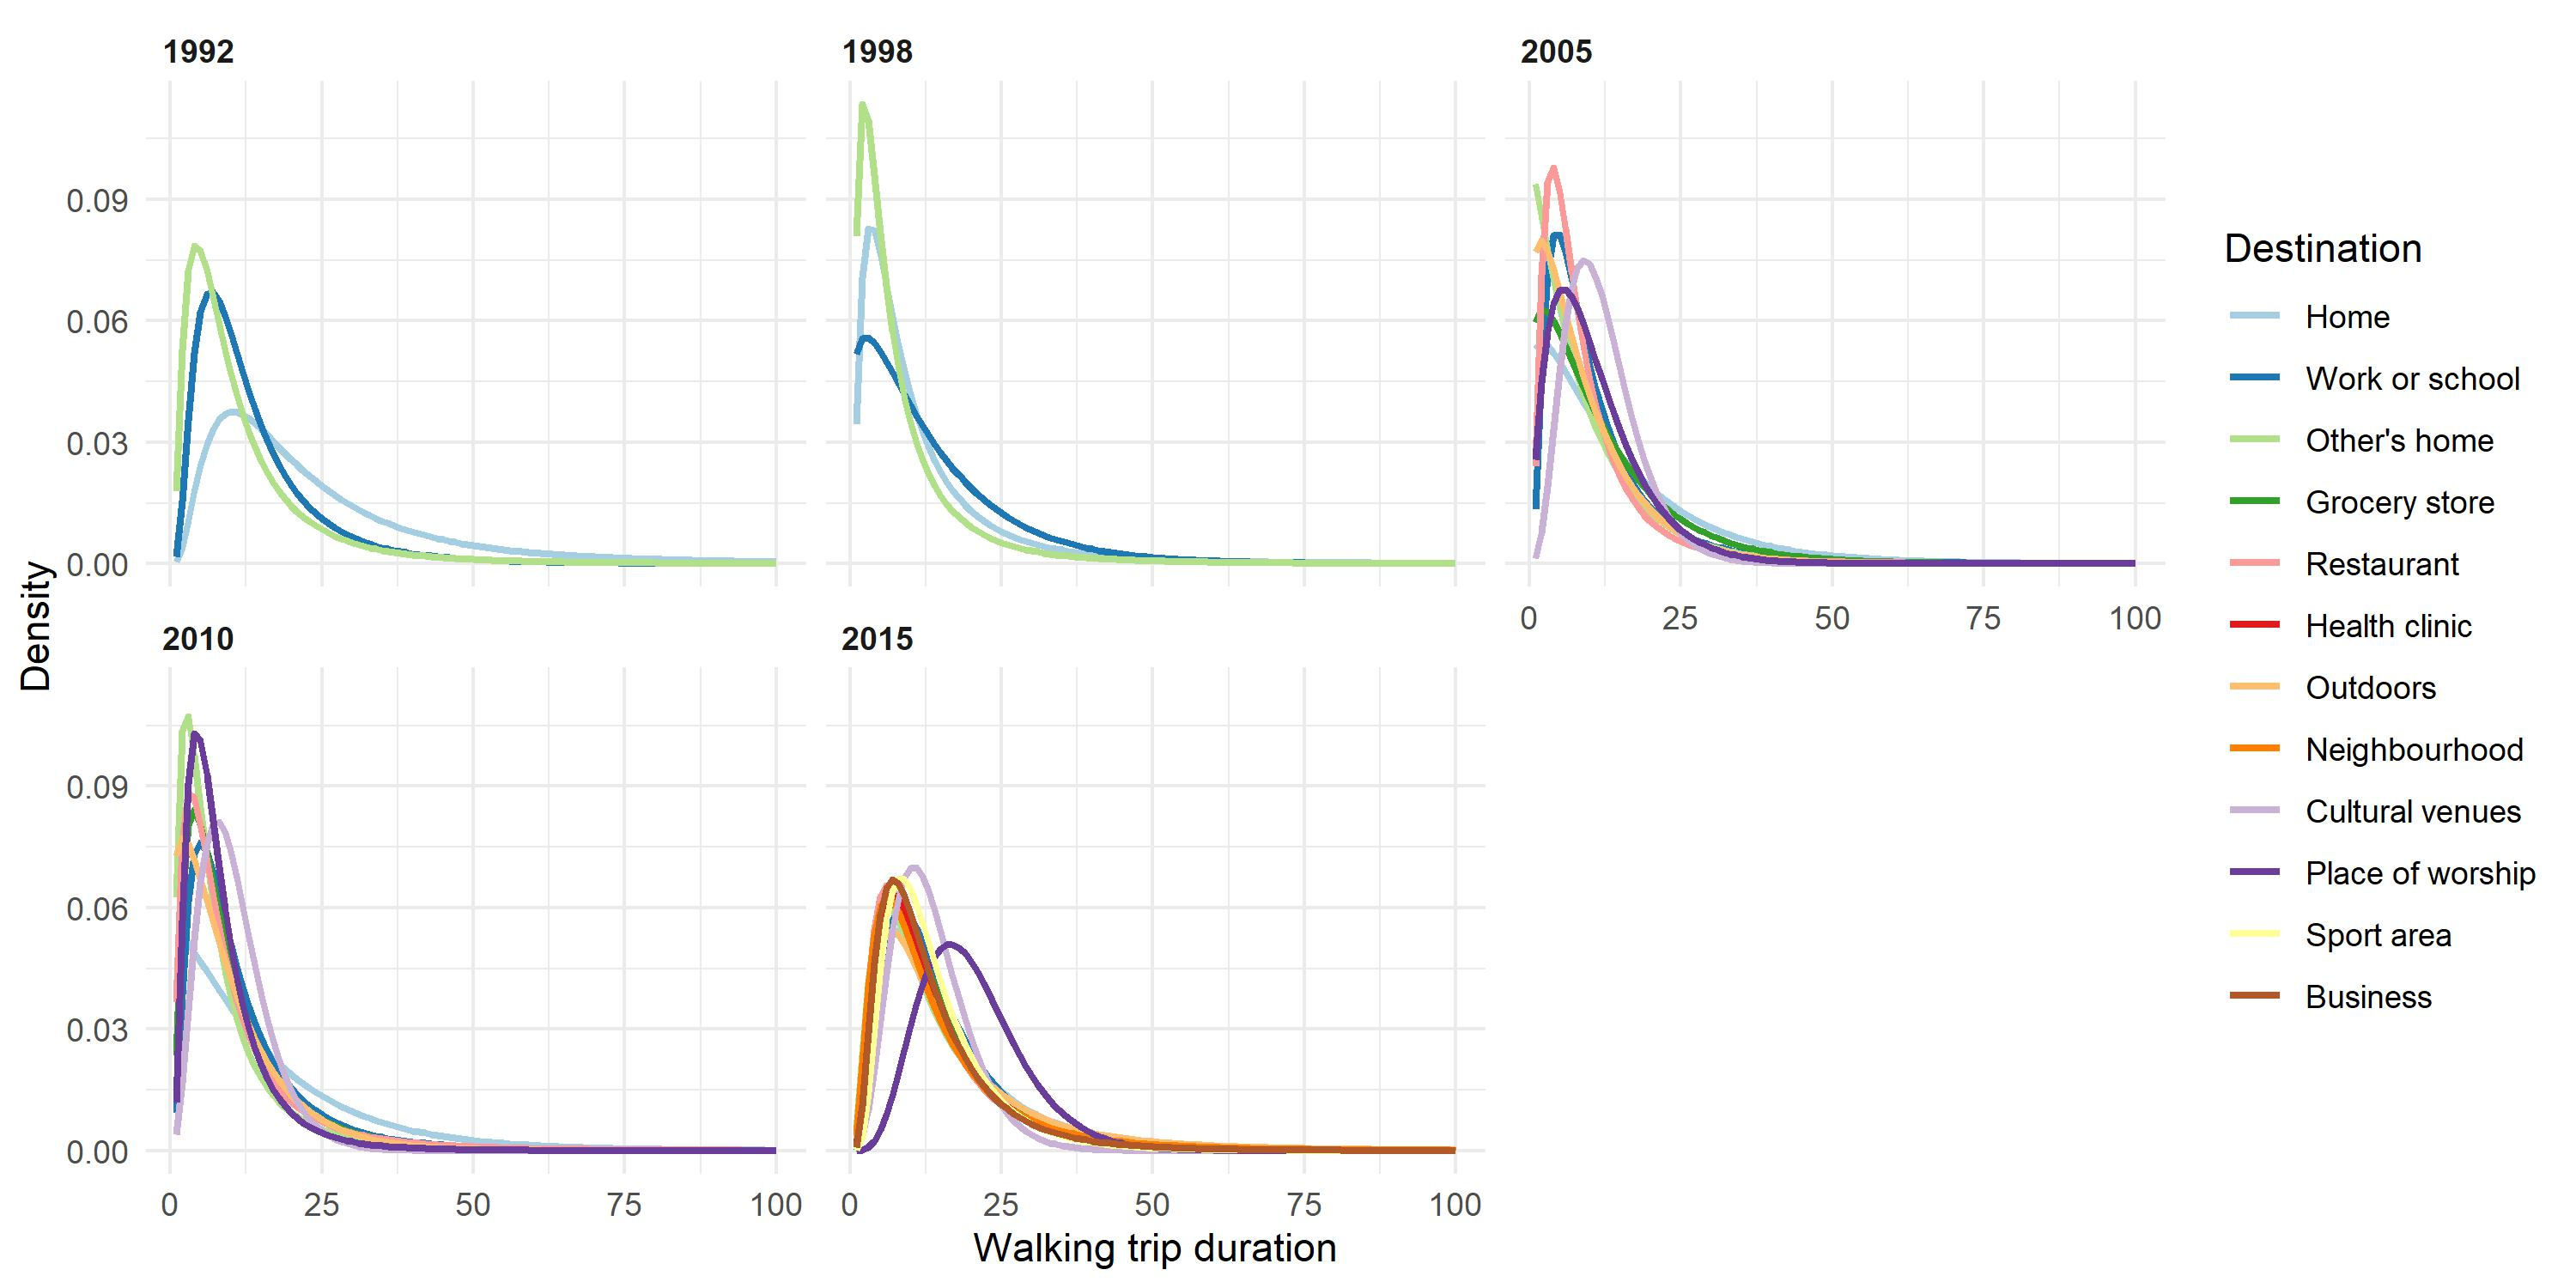
\includegraphics[width=1\linewidth]{figures/walking_functions_by_year} 

}

\caption{Walking functions grouped by year.}\label{fig:walking-function-by-year-fig}
\end{figure}

\begin{figure}

{\centering 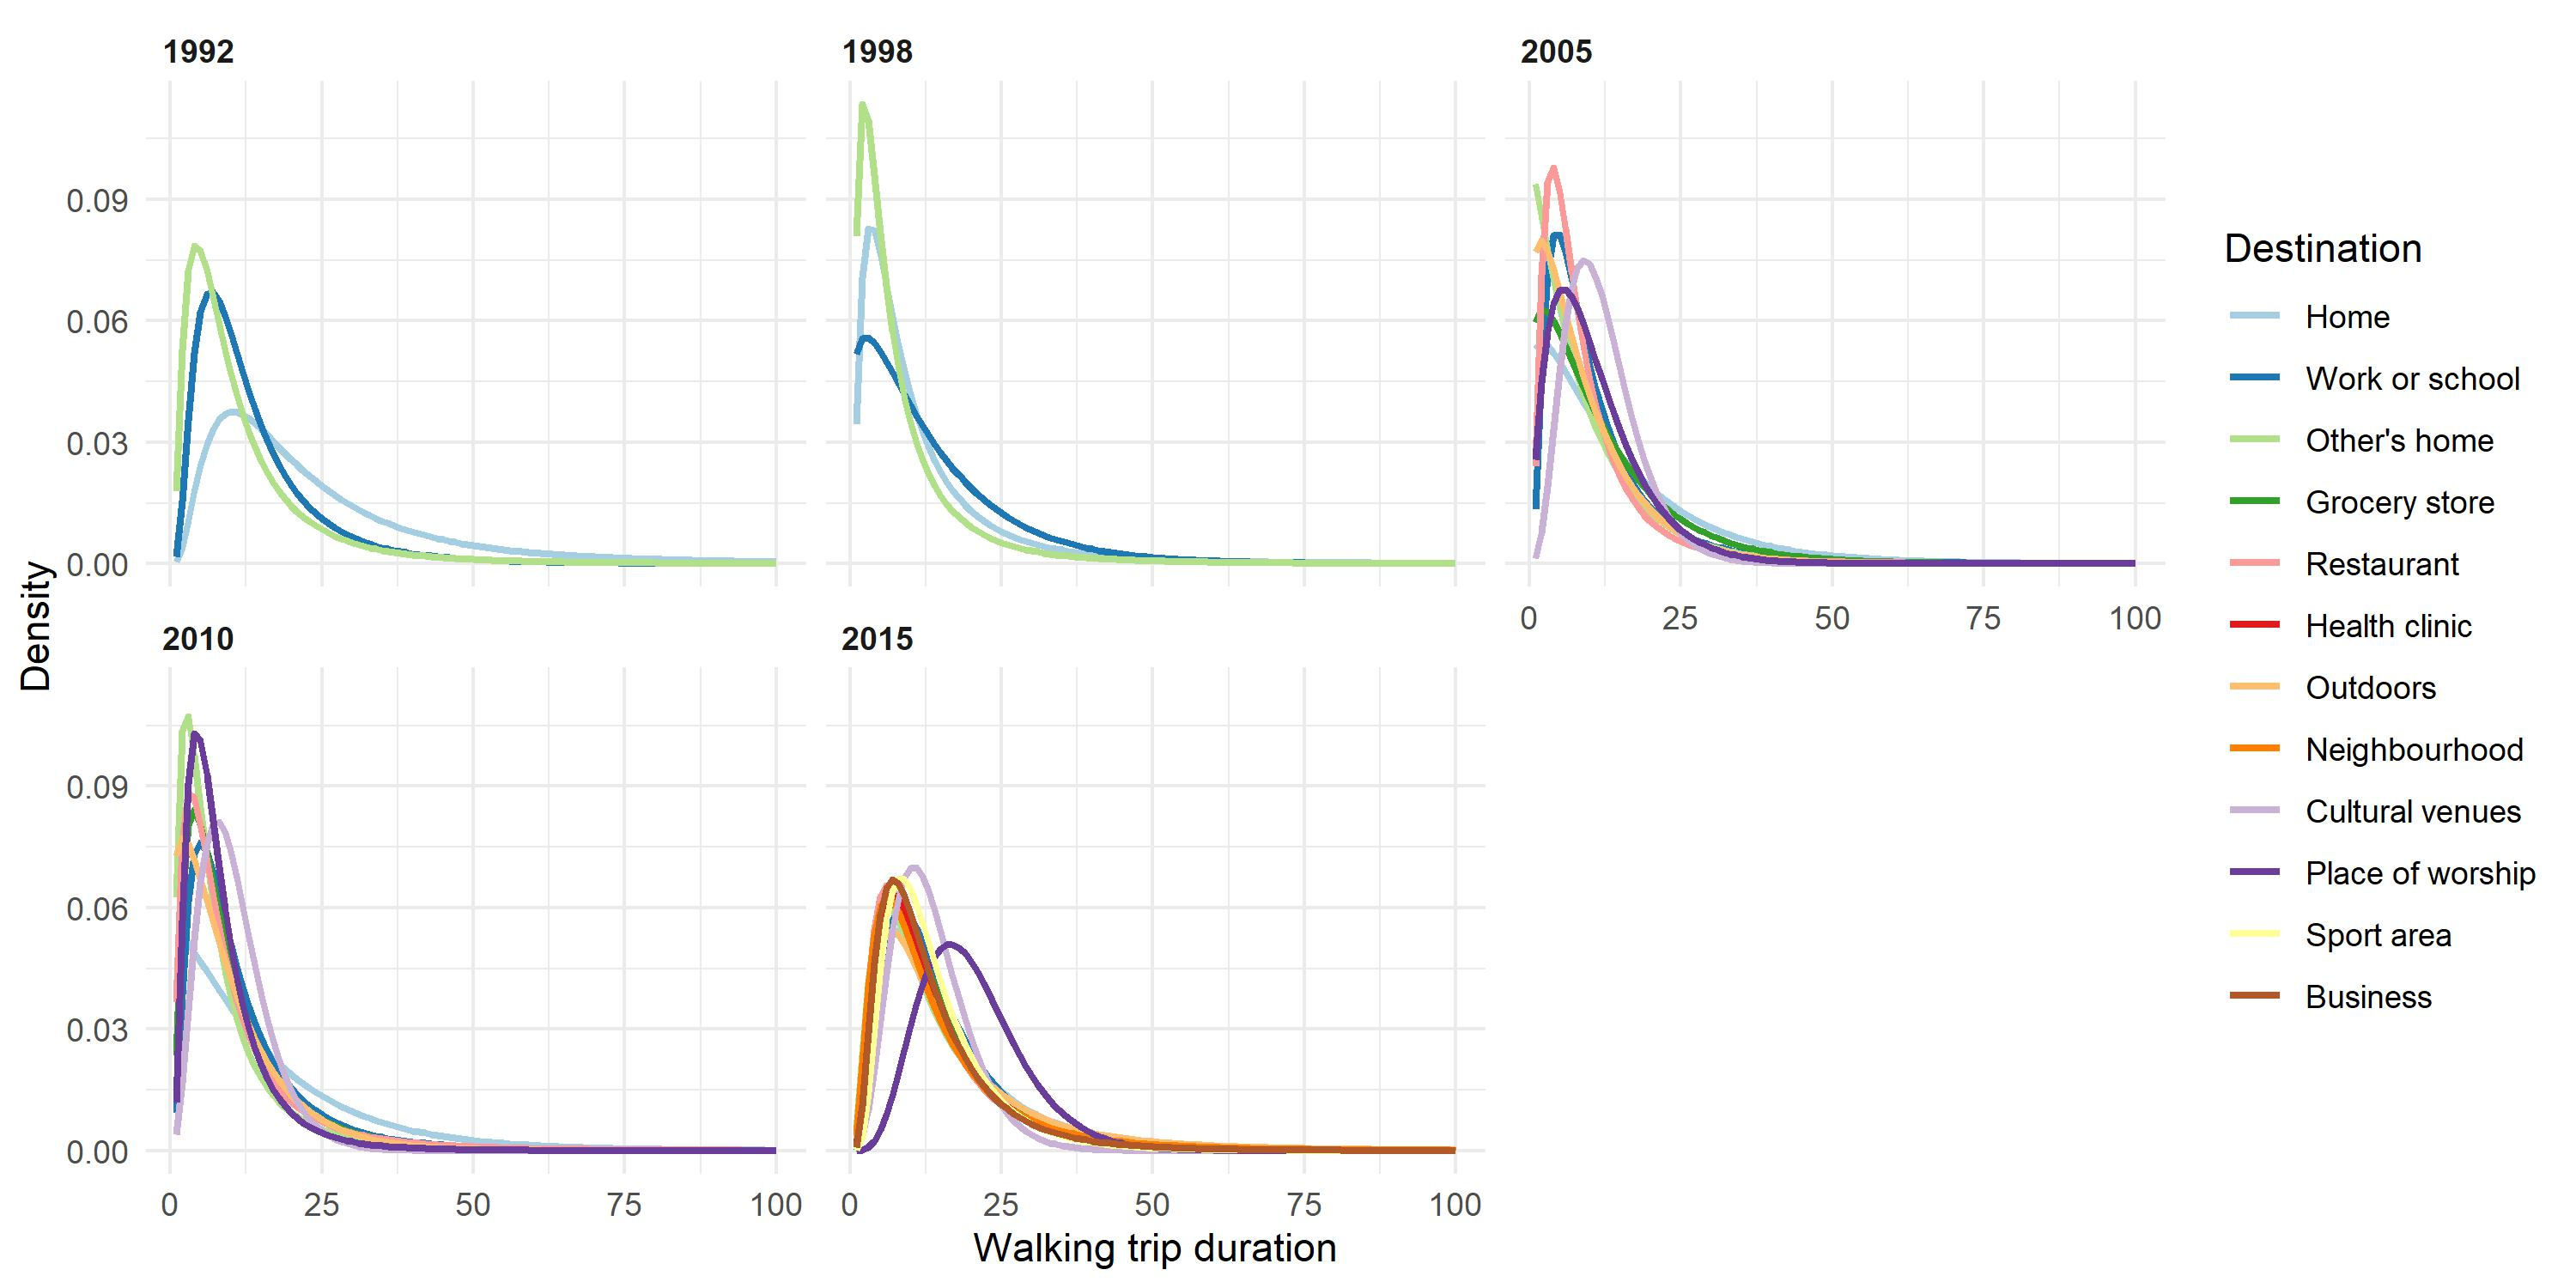
\includegraphics[width=1\linewidth]{figures/cycling_functions_by_year} 

}

\caption{Cycling functions grouped by year.}\label{fig:cycling-function-by-year-fig}
\end{figure}

\hypertarget{conclusion}{%
\subsection{Conclusion}\label{conclusion}}

\hypertarget{references}{%
\section*{References}\label{references}}
\addcontentsline{toc}{section}{References}

\hypertarget{refs}{}
\begin{CSLReferences}{1}{0}
\leavevmode\vadjust pre{\hypertarget{ref-apparicio2008comparing}{}}%
Apparicio, Philippe, Mohamed Abdelmajid, Mylene Riva, and Richard
Shearmur. 2008. {``Comparing Alternative Approaches to Measuring the
Geographical Accessibility of Urban Health Services: Distance Types and
Aggregation-Error Issues.''} \emph{International Journal of Health
Geographics} 7 (1): 1--14.

\leavevmode\vadjust pre{\hypertarget{ref-arranz2019measuring}{}}%
Arranz-Lopez, Aldo, Julio A Soria-Lara, Frank Witlox, and Antonio Paez.
2019. {``Measuring Relative Non-Motorized Accessibility to Retail
Activities.''} \emph{International Journal of Sustainable
Transportation} 13 (9): 639--51.

\leavevmode\vadjust pre{\hypertarget{ref-bhat2002development}{}}%
Bhat, Chandra, Susan Handy, Kara Kockelman, Hani Mahmassani, Anand
Gopal, Issam Srour, and Lisa Weston. 2002. {``Development of an Urban
Accessibility Index: Formulations, Aggregation, and Application.''}
\emph{Work} 4938 (4).

\leavevmode\vadjust pre{\hypertarget{ref-carrothers1956historical}{}}%
Carrothers, Gerald AP. 1956. {``An Historical Review of the Gravity and
Potential Concepts of Human Interaction.''} \emph{Journal of the
American Institute of Planners} 22 (2): 94--102.

\leavevmode\vadjust pre{\hypertarget{ref-cascetta2013new}{}}%
Cascetta, Ennio, Armando Carteni, and Marcello Montanino. 2013. {``A New
Measure of Accessibility Based on Perceived Opportunities.''}
\emph{Procedia-Social and Behavioral Sciences} 87: 117--32.

\leavevmode\vadjust pre{\hypertarget{ref-church2003measuring}{}}%
Church, Richard L, and James R Marston. 2003. {``Measuring Accessibility
for People with a Disability.''} \emph{Geographical Analysis} 35 (1):
83--96.

\leavevmode\vadjust pre{\hypertarget{ref-clifton2001evaluating}{}}%
Clifton, KELLY J, and SL Handy. 2001. {``Evaluating Neighborhood
Accessibility: Possibilities and Practicalities.''} \emph{Journal of
Transportation and Statistics} 4 (2-3): 67.

\leavevmode\vadjust pre{\hypertarget{ref-currie2010quantifying}{}}%
Currie, Graham. 2010. {``Quantifying Spatial Gaps in Public Transport
Supply Based on Social Needs.''} \emph{Journal of Transport Geography}
18 (1): 31--41.

\leavevmode\vadjust pre{\hypertarget{ref-de2009exponential}{}}%
De Vries, Jacob J, Peter Nijkamp, and Piet Rietveld. 2009.
{``Exponential or Power Distance-Decay for Commuting? An Alternative
Specification.''} \emph{Environment and Planning A} 41 (2): 461--80.

\leavevmode\vadjust pre{\hypertarget{ref-dunn2023}{}}%
Dunn, William L., and J. Kenneth Shultis. 2023. {``Appendix a - Some
Common Probability Distributions.''} In, edited by William L. Dunn and
J. Kenneth Shultis, 447--95. Elsevier.
\url{https://doi.org/10.1016/B978-0-12-819739-4.00019-6}.

\leavevmode\vadjust pre{\hypertarget{ref-eldridge1991warped}{}}%
Eldridge, J Douglas, and John Paul Jones III. 1991. {``Warped Space: A
Geography of Distance Decay.''} \emph{The Professional Geographer} 43
(4): 500--511.

\leavevmode\vadjust pre{\hypertarget{ref-fotheringham1981spatial}{}}%
Fotheringham, A Stewart. 1981. {``Spatial Structure and Distance-Decay
Parameters.''} \emph{Annals of the Association of American Geographers}
71 (3): 425--36.

\leavevmode\vadjust pre{\hypertarget{ref-fotheringham1989spatial}{}}%
Fotheringham, A Stewart, and Morton E O'Kelly. 1989. \emph{Spatial
Interaction Models: Formulations and Applications}. Vol. 1. Kluwer
Academic Publishers Dordrecht.

\leavevmode\vadjust pre{\hypertarget{ref-frank2001built}{}}%
Frank, Lawrence D, and Peter O Engelke. 2001. {``The Built Environment
and Human Activity Patterns: Exploring the Impacts of Urban Form on
Public Health.''} \emph{Journal of Planning Literature} 16 (2): 202--18.

\leavevmode\vadjust pre{\hypertarget{ref-frank2005linking}{}}%
Frank, Lawrence D, Thomas L Schmid, James F Sallis, James Chapman, and
Brian E Saelens. 2005. {``Linking Objectively Measured Physical Activity
with Objectively Measured Urban Form: Findings from SMARTRAQ.''}
\emph{American Journal of Preventive Medicine} 28 (2): 117--25.

\leavevmode\vadjust pre{\hypertarget{ref-geurs2006accessibility}{}}%
Geurs, Karst. 2006. \emph{Accessibility, Land Use and Transport:
Accessibility Evaluation of Land-Use and Transport Developments and
Policy Strategy}. Eburon Uitgeverij BV.

\leavevmode\vadjust pre{\hypertarget{ref-geurs2001accessibility}{}}%
Geurs, Karst T, and Jan R Ritsema van Eck. 2001. {``Accessibility
Measures: Review and Applications. Evaluation of Accessibility Impacts
of Land-Use Transportation Scenarios, and Related Social and Economic
Impact.''} \emph{RIVM Rapport 408505006}.

\leavevmode\vadjust pre{\hypertarget{ref-geurs2004}{}}%
Geurs, Karst T, and Bert Van Wee. 2004. {``Accessibility Evaluation of
Land-Use and Transport Strategies: Review and Research Directions.''}
\emph{Journal of Transport Geography} 12 (2): 127--40.

\leavevmode\vadjust pre{\hypertarget{ref-grengs2015nonwork}{}}%
Grengs, Joe. 2015. {``Nonwork Accessibility as a Social Equity
Indicator.''} \emph{International Journal of Sustainable Transportation}
9 (1): 1--14.

\leavevmode\vadjust pre{\hypertarget{ref-gutierrez1996european}{}}%
Gutierrez, Javier, Rafael Gonzalez, and Gabriel Gomez. 1996. {``The
European High-Speed Train Network: Predicted Effects on Accessibility
Patterns.''} \emph{Journal of Transport Geography} 4 (4): 227--38.

\leavevmode\vadjust pre{\hypertarget{ref-handy1993regional}{}}%
Handy, Susan. 1993. {``Regional Versus Local Accessibility: Implications
for Nonwork Travel.''}

\leavevmode\vadjust pre{\hypertarget{ref-handy1997measuring}{}}%
Handy, Susan L, and Debbie A Niemeier. 1997. {``Measuring Accessibility:
An Exploration of Issues and Alternatives.''} \emph{Environment and
Planning A} 29 (7): 1175--94.

\leavevmode\vadjust pre{\hypertarget{ref-hansen1959accessibility}{}}%
Hansen, Walter G. 1959. {``How Accessibility Shapes Land Use.''}
\emph{Journal of the American Institute of Planners} 25 (2): 73--76.

\leavevmode\vadjust pre{\hypertarget{ref-hino2014built}{}}%
Hino, Adriano AF, Rodrigo S Reis, Olga L Sarmiento, Diana C Parra, and
Ross C Brownson. 2014. {``Built Environment and Physical Activity for
Transportation in Adults from Curitiba, Brazil.''} \emph{Journal of
Urban Health} 91: 446--62.

\leavevmode\vadjust pre{\hypertarget{ref-hsiao1997use}{}}%
Hsiao, Shirley, Jian Lu, James Sterling, and Matthew Weatherford. 1997.
{``Use of Geographic Information System for Analysis of Transit
Pedestrian Access.''} \emph{Transportation Research Record} 1604 (1):
50--59.

\leavevmode\vadjust pre{\hypertarget{ref-hull2012accessibility}{}}%
Hull, Angela, Cecilia Silva, and Luca Bertolini. 2012.
\emph{Accessibility Instruments for Planning Practice}. Cost Office
Brussels.

\leavevmode\vadjust pre{\hypertarget{ref-iacono2010}{}}%
Iacono, Michael, Kevin J Krizek, and Ahmed El-Geneidy. 2010.
{``Measuring Non-Motorized Accessibility: Issues, Alternatives, and
Execution.''} \emph{Journal of Transport Geography} 18 (1): 133--40.

\leavevmode\vadjust pre{\hypertarget{ref-iacono2008access}{}}%
Iacono, Michael, Kevin Krizek, and Ahmed M El-Geneidy. 2008. {``Access
to Destinations: How Close Is Close Enough? Estimating Accurate Distance
Decay Functions for Multiple Modes and Different Purposes.''}

\leavevmode\vadjust pre{\hypertarget{ref-itf2017linking}{}}%
ITF. 2017. \emph{Linking People and Places: New Ways of Understanding
Spatial Access in Cities}. OECD Publishing.

\leavevmode\vadjust pre{\hypertarget{ref-kanafani1983transportation}{}}%
Kanafani, Adib. 1983. {``Transportation Demand Analysis.''}

\leavevmode\vadjust pre{\hypertarget{ref-koenig1980indicators}{}}%
Koenig, Jean-Gerard. 1980. {``Indicators of Urban Accessibility: Theory
and Application.''} \emph{Transportation} 9 (2): 145--72.

\leavevmode\vadjust pre{\hypertarget{ref-krizek2005perspectives}{}}%
Krizek, Kevin J. 2005. {``Perspectives on Accessibility and Travel.''}
In \emph{Access to Destinations}, 109--30. Emerald Group Publishing
Limited.

\leavevmode\vadjust pre{\hypertarget{ref-kwan1998space}{}}%
Kwan, Mei-Po. 1998. {``Space-Time and Integral Measures of Individual
Accessibility: A Comparative Analysis Using a Point-Based Framework.''}
\emph{Geographical Analysis} 30 (3): 191--216.

\leavevmode\vadjust pre{\hypertarget{ref-kwan2003recent}{}}%
Kwan, Mei-Po, Alan T Murray, Morton E OKelly, and Michael Tiefelsdorf.
2003. {``Recent Advances in Accessibility Research: Representation,
Methodology and Applications.''} \emph{Journal of Geographical Systems}
5: 129--38.

\leavevmode\vadjust pre{\hypertarget{ref-lamiquiz2015effects}{}}%
Lamiquiz, Patxi J, and Jorge Lopez-Dominguez. 2015. {``Effects of Built
Environment on Walking at the Neighbourhood Scale. A New Role for Street
Networks by Modelling Their Configurational Accessibility?''}
\emph{Transportation Research Part A: Policy and Practice} 74: 148--63.

\leavevmode\vadjust pre{\hypertarget{ref-larsen2010beyond}{}}%
Larsen, Jacob, Ahmed El-Geneidy, and Farhana Yasmin. 2010. {``Beyond the
Quarter Mile: Re-Examining Travel Distances by Active Transportation.''}
\emph{Canadian Journal of Urban Research} 19 (1): 70--88.

\leavevmode\vadjust pre{\hypertarget{ref-levinson2005access}{}}%
Levinson, David M, and Kevin J Krizek. 2005. \emph{Access to
Destinations}. Elsevier Publishers.

\leavevmode\vadjust pre{\hypertarget{ref-li2020approach}{}}%
Li, Aoyong, Yizhe Huang, and Kay W Axhausen. 2020. {``An Approach to
Imputing Destination Activities for Inclusion in Measures of Bicycle
Accessibility.''} \emph{Journal of Transport Geography} 82: 102566.

\leavevmode\vadjust pre{\hypertarget{ref-lowry2012using}{}}%
Lowry, M, Daniel Callister, M Gresham, and B Moore. 2012. {``Using
Bicycle Level of Service to Assess Community-Wide Bikeability.''} In
\emph{91st Annual Meeting of the Transportation Research Board,
Washington, DC: Transportation Research Board}.

\leavevmode\vadjust pre{\hypertarget{ref-luoma1993threshold}{}}%
Luoma, Martti, Kauko Mikkonen, and Mauri Palomaki. 1993. {``The
Threshold Gravity Model and Transport Geography: How Transport
Development Influences the Distance-Decay Parameter of the Gravity
Model.''} \emph{Journal of Transport Geography} 1 (4): 240--47.

\leavevmode\vadjust pre{\hypertarget{ref-meyer1984urban}{}}%
Meyer, Michael D, and Eric J Miller. 1984. {``Urban Transportation
Planning: A Decision-Oriented Approach.''}

\leavevmode\vadjust pre{\hypertarget{ref-mikkonen1999parameters}{}}%
Mikkonen, Kauko, and Martti Luoma. 1999. {``The Parameters of the
Gravity Model Are Changing--How and Why?''} \emph{Journal of Transport
Geography} 7 (4): 277--83.

\leavevmode\vadjust pre{\hypertarget{ref-miller2005place}{}}%
Miller, Harvey J. 2005. {``Place-Based Versus People-Based
Accessibility.''} In \emph{Access to Destinations}, 63--89. Emerald
Group Publishing Limited.

\leavevmode\vadjust pre{\hypertarget{ref-millward2013active}{}}%
Millward, Hugh, Jamie Spinney, and Darren Scott. 2013.
{``Active-Transport Walking Behavior: Destinations, Durations,
Distances.''} \emph{Journal of Transport Geography} 28: 101--10.

\leavevmode\vadjust pre{\hypertarget{ref-nassir2016utility}{}}%
Nassir, Neema, Mark Hickman, Ali Malekzadeh, and Elnaz Irannezhad. 2016.
{``A Utility-Based Travel Impedance Measure for Public Transit Network
Accessibility.''} \emph{Transportation Research Part A: Policy and
Practice} 88: 26--39.

\leavevmode\vadjust pre{\hypertarget{ref-osth2016new}{}}%
Osth, John, Johan Lyhagen, and Aura Reggiani. 2016. {``A New Way of
Determining Distance Decay Parameters in Spatial Interaction Models with
Application to Job Accessibility Analysis in Sweden.''} \emph{European
Journal of Transport and Infrastructure Research} 16 (2).

\leavevmode\vadjust pre{\hypertarget{ref-paez2012measuring}{}}%
Paez, Antonio, Darren M Scott, and Catherine Morency. 2012. {``Measuring
Accessibility: Positive and Normative Implementations of Various
Accessibility Indicators.''} \emph{Journal of Transport Geography} 25:
141--53.

\leavevmode\vadjust pre{\hypertarget{ref-papa2012gravity}{}}%
Papa, Enrica, and Pierluigi Coppola. 2012. {``Gravity-Based
Accessibility Measures for Integrated Transport-Land Use Planning
(GraBAM).''} \emph{Accessibility Instruments for Planning Practice} 117:
124.

\leavevmode\vadjust pre{\hypertarget{ref-pirie1979measuring}{}}%
Pirie, Gordon H. 1979. {``Measuring Accessibility: A Review and
Proposal.''} \emph{Environment and Planning A} 11 (3): 299--312.

\leavevmode\vadjust pre{\hypertarget{ref-prins2014many}{}}%
Prins, Richard G, Frank Pierik, Astrid Etman, Reinier P Sterkenburg,
Carlijn BM Kamphuis, and FJ Van Lenthe. 2014. {``How Many Walking and
Cycling Trips Made by Elderly Are Beyond Commonly Used Buffer Sizes:
Results from a GPS Study.''} \emph{Health \& Place} 27: 127--33.

\leavevmode\vadjust pre{\hypertarget{ref-reggiani2011accessibility}{}}%
Reggiani, Aura, Pietro Bucci, and Giovanni Russo. 2011. {``Accessibility
and Impedance Forms: Empirical Applications to the German Commuting
Network.''} \emph{International Regional Science Review} 34 (2):
230--52.

\leavevmode\vadjust pre{\hypertarget{ref-saghapour2017measuring}{}}%
Saghapour, Tayebeh, Sara Moridpour, and Russell G Thompson. 2017.
{``Measuring Cycling Accessibility in Metropolitan Areas.''}
\emph{International Journal of Sustainable Transportation} 11 (5):
381--94.

\leavevmode\vadjust pre{\hypertarget{ref-sallis2004active}{}}%
Sallis, James F, Lawrence D Frank, Brian E Saelens, and M Katherine
Kraft. 2004. {``Active Transportation and Physical Activity:
Opportunities for Collaboration on Transportation and Public Health
Research.''} \emph{Transportation Research Part A: Policy and Practice}
38 (4): 249--68.

\leavevmode\vadjust pre{\hypertarget{ref-signorino2011gravity}{}}%
Signorino, Guido, Roberto Pasetto, Elisa Gatto, Massimo Mucciardi,
Marina La Rocca, and Pierpaolo Mudu. 2011. {``Gravity Models to Classify
Commuting Vs. Resident Workers. An Application to the Analysis of
Residential Risk in a Contaminated Area.''} \emph{International Journal
of Health Geographics} 10 (1): 1--10.

\leavevmode\vadjust pre{\hypertarget{ref-skov2001estimation}{}}%
Skov-Petersen, Hans. 2001. {``Estimation of Distance-Decay Parameters:
GIS-Based Indicators of Recreational Accessibility.''} In
\emph{ScanGIS}, 237--58.

\leavevmode\vadjust pre{\hypertarget{ref-song1996some}{}}%
Song, Shunfeng. 1996. {``Some Tests of Alternative Accessibility
Measures: A Population Density Approach.''} \emph{Land Economics},
474--82.

\leavevmode\vadjust pre{\hypertarget{ref-sun2012measuring}{}}%
Sun, Guibo, Hui Lin, and Rongrong Li. 2012. {``Measuring the Influence
of Built Environment on Walking Behavior: An Accessibility Approach.''}
In \emph{Geographic Information Science: 7th International Conference,
GIScience 2012, Columbus, OH, USA, September 18-21, 2012. Proceedings
7}, 187--97. Springer.

\leavevmode\vadjust pre{\hypertarget{ref-taylor1975distance}{}}%
Taylor, Peter. 1975. {``Distance Decay Models in Spatial
Interactions.''} \emph{(No Title)}.

\leavevmode\vadjust pre{\hypertarget{ref-untermann1984accommodating}{}}%
Untermann, Richard K. 1984. {``Accommodating the Pedestrian: Adapting
Towns and Neighbourhoods for Walking and Bicycling.''}

\leavevmode\vadjust pre{\hypertarget{ref-vale2017influence}{}}%
Vale, David S, and Mauro Pereira. 2017. {``The Influence of the
Impedance Function on Gravity-Based Pedestrian Accessibility Measures: A
Comparative Analysis.''} \emph{Environment and Planning B: Urban
Analytics and City Science} 44 (4): 740--63.

\leavevmode\vadjust pre{\hypertarget{ref-vandenbulcke2009mapping}{}}%
Vandenbulcke, Gregory, Therese Steenberghen, and Isabelle Thomas. 2009.
{``Mapping Accessibility in Belgium: A Tool for Land-Use and Transport
Planning?''} \emph{Journal of Transport Geography} 17 (1): 39--53.

\leavevmode\vadjust pre{\hypertarget{ref-vasconcelos2012evaluation}{}}%
Vasconcelos, Ana S, and Tiago L Farias. 2012. {``Evaluation of Urban
Accessibility Indicators Based on Internal and External Environmental
Costs.''} \emph{Transportation Research Part D: Transport and
Environment} 17 (6): 433--41.

\leavevmode\vadjust pre{\hypertarget{ref-vega2012using}{}}%
Vega, Amaya. 2012. {``Using Place Rank to Measure Sustainable
Accessibility.''} \emph{Journal of Transport Geography} 24: 411--18.

\leavevmode\vadjust pre{\hypertarget{ref-vickerman1974accessibility}{}}%
Vickerman, Roger W. 1974. {``Accessibility, Attraction, and Potential: A
Review of Some Concepts and Their Use in Determining Mobility.''}
\emph{Environment and Planning A} 6 (6): 675--91.

\leavevmode\vadjust pre{\hypertarget{ref-wu2019measuring}{}}%
Wu, Xueying, Yi Lu, Yaoyu Lin, and Yiyang Yang. 2019. {``Measuring the
Destination Accessibility of Cycling Transfer Trips in Metro Station
Areas: A Big Data Approach.''} \emph{International Journal of
Environmental Research and Public Health} 16 (15): 2641.

\leavevmode\vadjust pre{\hypertarget{ref-yang2012walking}{}}%
Yang, Yong, and Ana V Diez-Roux. 2012. {``Walking Distance by Trip
Purpose and Population Subgroups.''} \emph{American Journal of
Preventive Medicine} 43 (1): 11--19.

\leavevmode\vadjust pre{\hypertarget{ref-zhao2003forecasting}{}}%
Zhao, Fang, Lee-Fang Chow, Min-Tang Li, Ike Ubaka, and Albert Gan. 2003.
{``Forecasting Transit Walk Accessibility: Regression Model Alternative
to Buffer Method.''} \emph{Transportation Research Record} 1835 (1):
34--41.

\end{CSLReferences}


\end{document}
